\documentclass[]{report}

% Package to allow utf8 characters (needed for umlauts)
\usepackage[utf8]{inputenc}

% Packacge for including images
\usepackage{graphicx}
\graphicspath{{graphics/}}

% Show sub sub sections in the contents
\setcounter{tocdepth}{3}

% Package for displaying maths stuff
\usepackage{mathtools}

% Packages for positioning Figures
\usepackage{float}
\usepackage{subcaption}

% Package for quotes
\usepackage{dirtytalk}

% Package for appenices
\usepackage{appendix}

% Package to hyperlink references
\usepackage{hyperref}

% Command for multi lining table cells
\newcommand{\specialcell}[2][c]{%
	\begin{tabular}[#1]{@{}c@{}}#2\end{tabular}}

% Title Page
\title{
	A Game Building Framework and SwingGame\endgraf
	Third Year Project Report
}
\author{
	\parbox{\linewidth}{
		\centering%
		Tim Brier\endgraf
		School of Computer Science\endgraf
		University of Manchester
	}
}
% Abuse the date to add extra info to the title page
\date{
	\parbox{\linewidth}{
		\centering%
		April 2015\endgraf\bigskip
		Supervised by Dr Steve Pettifer
	}
}


\begin{document}

\maketitle

\begin{abstract}
This paper details the development of SwingGame, a 2D video game in which players use ropes and grappling hooks to get to a goal in various levels.  The SwingGame project had two main goals, to produce a reusable framework for building games and to produce a fun and engaging game using that framework. The goals were successfully achieved with the framework being used for multiple finished products and SwingGame receiving praise by those who have seen and played it.

For the full source code of SwingGame and the framework as it was built for SwingGame visit \url{https://www.github.com/sizlo/SwingGame} and for ongoing development to the game framework visit \url{https://www.github.com/sizlo/TimGameLib}.
\end{abstract}

\tableofcontents

\chapter{Introduction}
This idea behind this project was to produce a framework for creating games and a game which uses that framework. The framework was to be generic and be able to facilitate the making of many different types of games. Eventually the framework may be used to produce commercial games but initially it will be used for personal projects as an effort to become better at making games.

SwingGame is the game which was produced alongside this framework to prove that the framework works. It is a 2D game in which a player must get from a starting point to a goal point in many levels. The only way to achieve this is by using several different types of swings which can be attached to obstacles within the level. Figure \ref{sgexample} shows a player swinging towards the goal in one of the levels of SwingGame.

\begin{figure}[H]
	\centerline{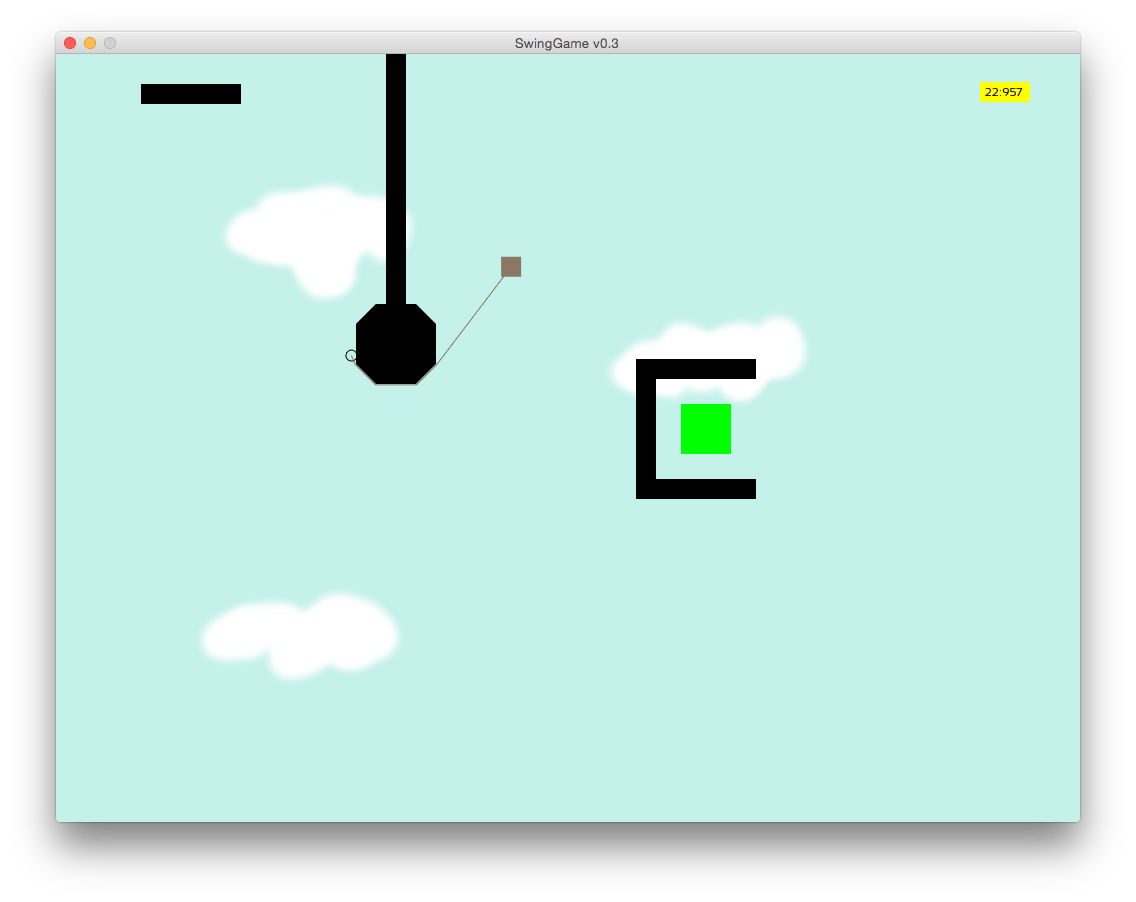
\includegraphics[width=1.5\textwidth]{sgexample}}
	\caption{Level 4 of SwingGame. The brown square is the player, the black shapes are obstacles and the green square is the goal.}
	\label{sgexample}
\end{figure}

\chapter{Context}
This chapter provides an overview of what the project contains and its main goals. Similar existing technology is discussed along with why the decision to make a new system was made.
	\section{Project Description}
	The main system produced in this project is the game framework. This framework should handle all tasks generic to every video game including window management, drawing to the window and event handling. The framework should be easy to use, a developer should be able to define just the level and player behaviour and have a working game. It should also be extensible so that if any future projects require more complex features they can be easily added in.
	
	SwingGame was built using and alongside this framework. The game consists of a number of levels, each containing several obstacles and a goal. The aim of each level is to travel from the players starting point to the goal of the level using the physics of swinging around the various obstacles. Levels are scored based on the time it took for the player to reach the goal. The main objective of SwingGame is to show that the game framework is usable, but ideally it should also be an entertaining and engaging game.
	\section{Existing Technologies}
	This Section discusses existing technology similar to this project. The technologies include other game frameworks and existing games which incorporate similar swinging mechanics.
		\subsection{Game Frameworks}
		There already exists several game frameworks (sometimes called engines) which have a variety of different feature sets. The most popular and most similar of these frameworks are discussed here.
			\subsubsection{Popular Frameworks}
			The most popular publicly available frameworks in use today are Unity \cite{unity} and Unreal Engine \cite{unreal}. Both of these frameworks are extremely powerful and complex. They focus more on 3D environments, providing systems to create game worlds and accurate real world physics simulation. These engines have historically been used in large projects with teams of developers but are now starting to be adopted by single developers due to more relaxed licensing fees.
			\subsubsection{Similar Frameworks}
			GameMaker \cite{gamemaker} is a framework more similar to the one in this project in that it is used for 2D games but it is also a lot more complex. It provides an entire language for developers to use to create games and includes GUI systems which allow developers to make games with minimal coding.
			
			A much more similar framework to the one in this project is Löve \cite{love}. Löve allows developers to script the behaviour of 2D games in Lua and provides modules to handle common game tasks including drawing, event handling and physics.
			\subsubsection{Decision To Make A New Framework}
			Most of the frameworks discussed previously were too complex for the needs of SwingGame. This project did not need a whole suite of tools for creating worlds and animations so the most likely candidate to use was Löve. However the decision was made to create a new framework for the project, mostly as a learning exercise. The Dragonfly project shows that \say{game engines present the opportunity to strengthen programming skills and expose students to a range of fundamental computer science topics} \cite{dragonfly}. Also, the most interesting component of this project, implementation wise, was the physics of the game. If an existing physics system was used the SwingGame project would have been too simple.
			
		\subsection{Games}
		Several games exist which have similar swinging mechanics to SwingGame. This Section will discuss how some of those games use swinging and how they differ from SwingGame.
			\subsubsection{Spider-Man}
			Various Spider-Man games have used swinging on a web line to get around the environment, one of which is Spider-Man 2 \cite{spiderman} by Treyarch. In this game the player uses the swinging mechanic to quickly navigate around a 3D virtual New York City.
			
			\begin{figure}[H]
				\centering
				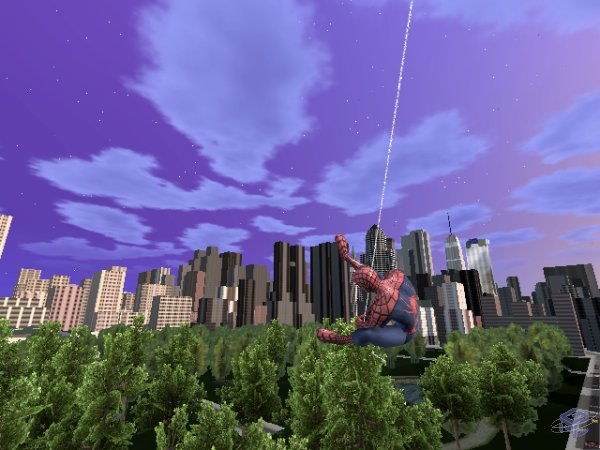
\includegraphics[scale=1.8]{spiderman}
				\caption{Web swinging in Spider-Man 2 \cite{spidermanimage}}
				\label{spidermanimage}
			\end{figure}
			\subsubsection{Worms}
			The Worms \cite{worms} series by Team17 includes an item called the Ninja Rope. This item is used to attach to scenery in the level and swing the character to areas that would have otherwise been inaccessible. The swinging in these games was the biggest inspiration for SwingGame so it behaves very similarly to the swinging in SwingGame.
			\begin{figure}[H]
				\centerline{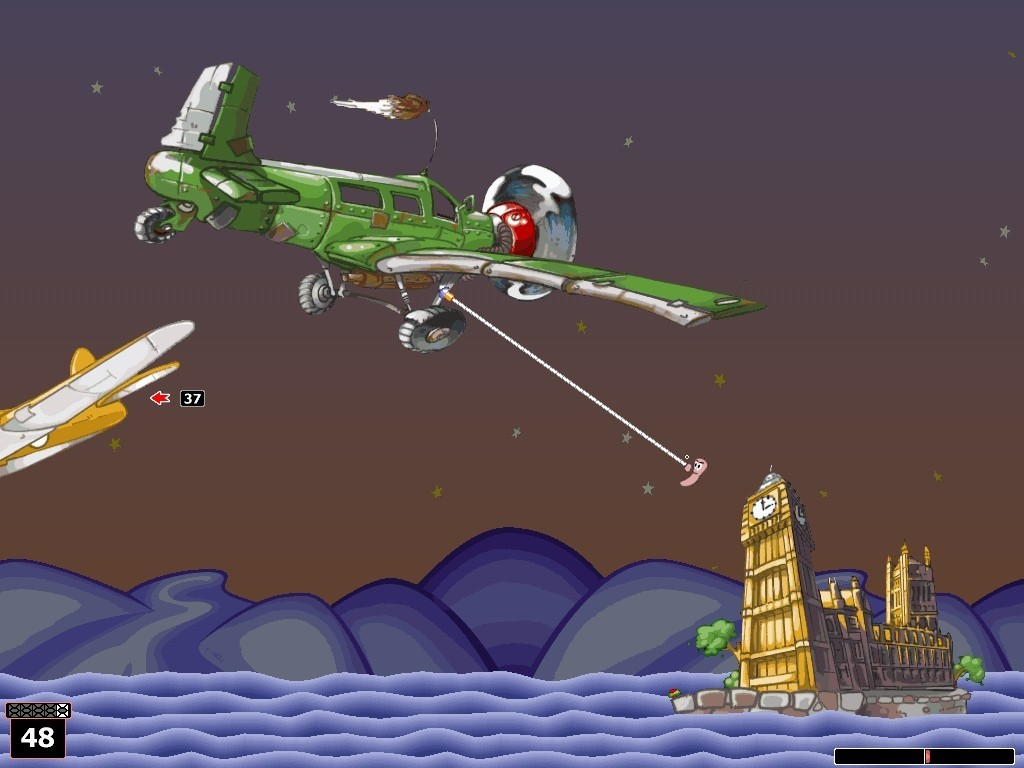
\includegraphics[width=0.75\textwidth]{worms}}
				\caption{The ninja rope in Worms Armageddon  \cite{wormsimage}}
				\label{wormsimage}
			\end{figure}
			\subsubsection{Floating Point}
			Floating Point \cite{floatingpoint} is a game by independent developer Tom Francis. This game is built upon using swinging to move around a 2D level, much like SwingGame. The player must use swinging to gain speed which makes several bars in the level grow taller. When the player crosses paths with one of these bars they collect points, the taller the bar the more points it scores.
			
			\begin{figure}[H]
				\centerline{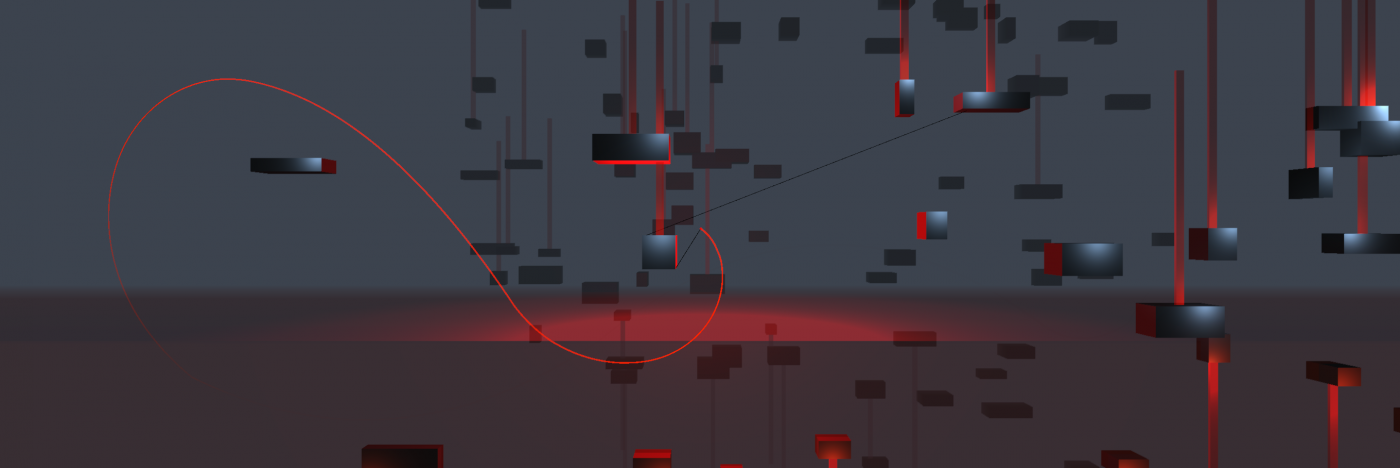
\includegraphics[width=1.5\textwidth]{floatingpoint}}
				\caption{Swinging around a block in Floating Point \cite{floatingpoint}}
				\label{floatingpointimage}
			\end{figure}
			\subsubsection{Differences With SwingGame}
			While the swinging movement in SwingGame is very similar to that of the Worms games and Floating Point it differs in objective to all of the discussed games. The other games all use swinging to move generally through the level and don't enforce a specific goal area. In SwingGame the entire aim of each level is to navigate around the various obstacles to reach one specific goal point in the level, making each level into a puzzle for the player to solve.

\chapter{Design}
This chapter details the design process of the project and the decisions made within it. The decisions for the requirements and technologies used for the framework are explained and a high level look at the game design is discussed.
	\section{Requirements}
	In this Section the requirements made for the game framework are discussed including the essential features and some more high level conventions.
		\subsection{Features}
		The game framework should ideally include as many features as possible which are needed in most games. Doing this would ensure that redundant code would not have to be written in multiple games. The following is a list of features which are essential to the game framework ranked in order of importance, one being the most important.
		\begin{enumerate}
			\item{Game loop}
			\item{Window management}
			\item{Drawing graphics}
			\item{Event management}
		\end{enumerate}
		All of these features are needed for a game to exist. A game needs to be built upon a game loop which controls its logic and it needs a window to display the game state in. It must be able to draw graphics in that window to show the current state and requires event management in order to respond to user input and make the game interactive. Each of these features is discussed in more depth in the next chapter.
		
		A list of features which are not essential to the framework but are still very useful is given below, ranked in order of most useful.
		\begin{enumerate}
			\item{Collision detection}
			\item{Physics}
			\item{Menu system}
			\item{Sound and music}
			\item{Animation}
		\end{enumerate}
		It was decided that the three most useful of these, collision detection, physics and a menu system would be added to the game framework while developing SwingGame. While audio and animation would have made SwingGame a better game they were far from the focus of the project. The intention was to add these features in if they were required for a future game.
		
		\subsection{Conventions}
		During the design of the framework some conventions were decided upon to be followed during development. One of these was to not expose underlying libraries used in the framework to the game in case it was ever decided to change these libraries. The framework should act as a layer of abstraction between the game and the libraries.
		
	\section{Technologies Used}
		This Section covers the different technologies used in the project.
		\subsection{Language}
		One of the aims of the game framework was to be platform agnostic so that it could be used to make games for any and all platforms. Because of this a good choice of language to use would have been Java, however C++ was used instead. The decision to use C++ was made because it is the industry standard language for writing games and by using it to create a game and a game framework I would be able to teach myself how to program in it more effectively.
		\subsection{Tools}
		A number of tools were used to facilitate this project. Development mainly took place in Xcode for OSX as I was very familiar with it while Windows builds were made in Visual Studio. Source control was handled by git and the entire project was hosted open source on GitHub.
		\subsection{Libraries}
		It was never the point of this project to handle different operating systems versions of window handles and event queues so it was decided that libraries would be used to handle the cross platform interfacing of these types of systems. A number of different libraries were researched and the following table shows a comparison of their features.
		
		\begin{figure}[H]
		\begin{tabular}[H]{ l || c | c | c }
			Feature & SFML 2.2 \cite{sfml} & SDL 2.0 \cite{sdl} & Allegro 5.1 \cite{allegro} \\
			\hline
			\hline
			Language & C++ & C & C \\
			Windows & Y & Y  & Y \\
			Events & Y & Y & Y \\
			2D Graphics & Y & Y & Y \\
			Audio & Y & Y & N \\
			Timing & Y & Y & Y \\
			Networking & Y & N & N \\
			Threading & Y & Y & Y \\
			\hline
			Windows Support & Y & Y & Y \\
			OSX Support & Y & Y & Y \\
			Linux Support & Y & Y & Y \\
			iOS Support & Y\footnotemark & Y & Y \\
			Android Support &Y\footnotemark[1] & Y & Y \\
		\end{tabular}
		\end{figure}
		
		\footnotetext{Experimental support in the current version}
		
		It was decided to use SFML 2.2 \cite{sfml} because not only was it more feature rich than the alternatives, but it also had a C++ object oriented interface compared to the straight C interface of the others. The caveat to this decision was that the mobile support for SFML was not as robust as the alternatives, but SwingGame was never intended to be a mobile game so this was not a major issue.
		
		The project was going to involve the use of XML files for storing levels so an XML parsing library was required. The decision was made to use pugixml \cite{pugixml} as it was a lightweight C++ library that had received praise on a number of forums.
		
		One more library was used which was a port of the dirent.h UNIX header for Visual  \cite{dirent}. This was used to allow SwingGame to traverse files in a directory with a simple API.
		
	\section{Game Design}
	This Section details some of the decisions made when designing the systems within SwingGame.
	\subsection{Objective}
	An objective had to be introduced in order for SwingGame to be a game. This objective could have taken multiple forms such as collecting items to build up a score or follow a particular path. The decision was made to have the player attempt to reach a specific point of the level, known as the goal, since this would allow flexibility in play styles (i.e goals could be reached in multiple ways).
	\subsection{Player Actions}
	The set of actions the player was able to do was kept quite small in order to keep the scope of SwingGame fairly small and manageable. What follows is the list of actions decided to be included in the game.
	\begin{itemize}
		\item{Attach a swing to an anchor}
		\item{Detach from a swing}
		\item{Jump from certain swings}
		\item{Climb and descend the rope of a swing}
		\item{Switch swing type}
	\end{itemize}
	Notice that every action involves a swing. This was intentional as it meant if the player was not swinging they had no control over themselves, forcing them to use the swinging system to complete the levels.
	\subsection{Other Thoughts}
	SwingGame was intended to focus on smooth and elegant swinging through a level so it was decided that the player would be punished heavily when they do something wrong. Because of this the decision was made to have the player lose a lot of their speed when they collide with an obstacle.
	
	The priority for the physics of the game was always for them to feel good, not to be completely accurate to the real world. The player enjoying swinging through the level was more important than the simulation being entirely perfect. This idea led me to change my mind about how physics would be implemented which is discussed in the next chapter.

\chapter{Development}
This chapter outlines the development process of the project. It discusses some decisions which were made during implementation and the modules created. Some implementation detail is provided for the more interesting parts of the project.

	\section{SFML Abstractions}
	As mentioned in the previous chapter it was decided that there should be a layer of abstraction between the game framework and SFML. One reason behind this was that it was always possible that the classes provided by SFML would be missing some desired functionality. By putting a layer in between the framework and SFML any extra features could be implemented in this layer. This proved to be useful for adding a pause feature to the provided clock class among other enhancements.
	
	The way this abstraction was implemented was to create a class for each SFML class the framework used. The created class inherited from the SFML class and all uses of the class in the framework would use the new subclass. This meant than whenever functionality was added to an SFML subclass this functionality could be used by any existing instance of the class in the project without having to change its type.
	
	\section{Modules}
	This Section details the various modules present in both the game framework and in SwingGame. A high level view of how each module works is provided as well as some of the more interesting details of the implementation.
		\subsection{Game Framework}
		The modules contained in the game framework are those which are not dependant on the type of game being made. Whatever the end product is these tasks will always be performed in the same way.
			\subsubsection{Graphics}
			The requirements for graphics in this project were fairly straightforward, draw shapes and text to the screen. The most advanced graphics feature was being able to load an image into an object called a sprite which can move around the screen. This was mostly handled by SFML but some extra features were implemented. An image cache was created meaning that multiple sprites could share the same loaded image instead of duplicating it in memory. The ability to draw debug features of shapes was also implemented. The graphics module could draw the origin of each shape along with all the points that make up that shape. A very useful piece of debug information which could be drawn was the bounding box of a shape, the smallest axis aligned rectangle which contains the entire shape. This bounding box is used in collisions and being able to see it proved very useful when working on collisions.
			\begin{figure}[H]
				\centering
				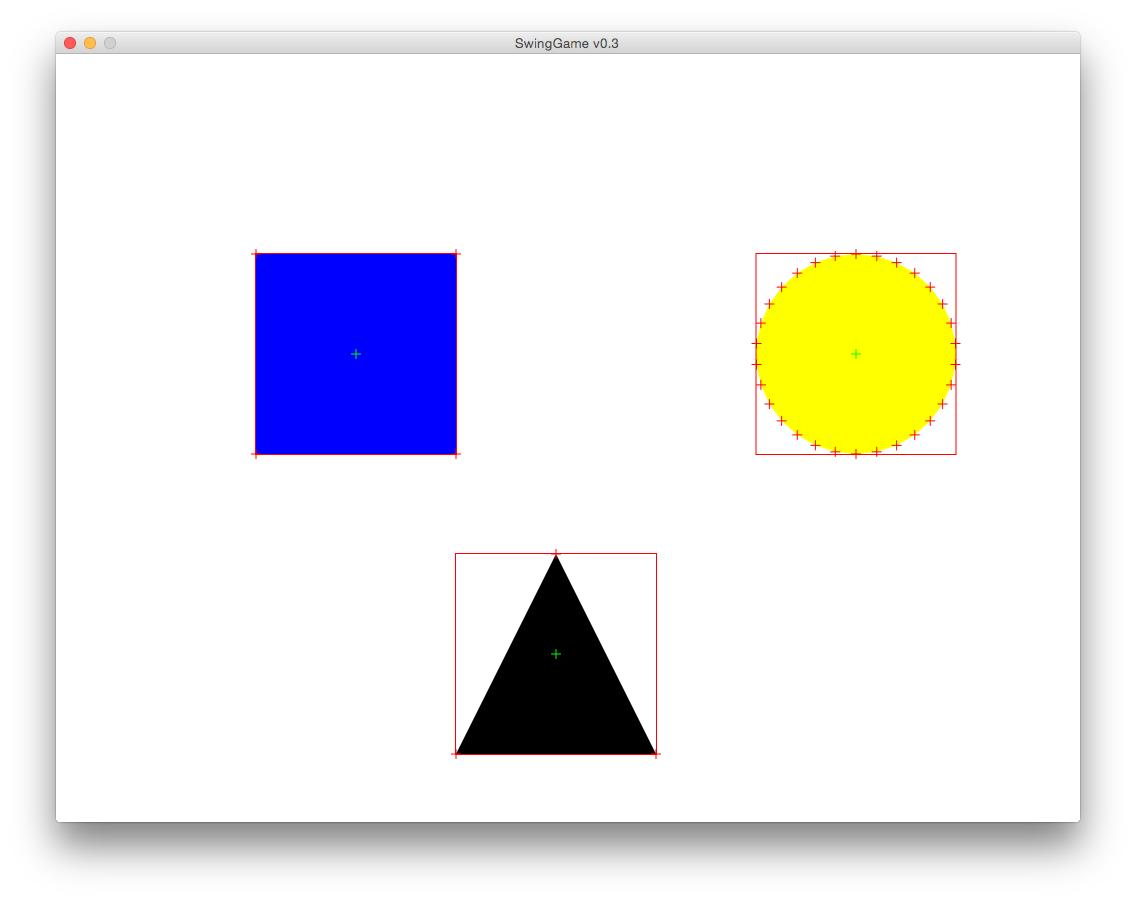
\includegraphics[scale=0.25]{debuggraphics}
				\caption{A simple scene with debug graphics being drawn}
				\label{debuggraphics}
			\end{figure}
			
			\subsubsection{Game Loop}
			Almost every video game runs on top of what is called a game loop. Inside this loop is where the gameplay logic is executed including updating the players position and handling any user input. One of the most important aspects of a game loop is that it must be non blocking since games are interactive. This means that instead of waiting for the next input event the game is constantly processing cycles of the loop and reacts to any events when they happen to come in. The loop \say{processes user input, but doesn’t wait for it} \cite{gamepatterns}.
			
			The game loop in this projects game framework does three things on every cycle:
			\begin{enumerate}
				\item Process events
				\item Update game objects
				\item Draw the current game state
			\end{enumerate}
			
			At different points of the games lifetime this loop needs to be processing different things. When the user is at a menu it should be updating the menu navigation and drawing the menu options with the current selection highlighted. When the user is in a level it should be updating the physics simulation and drawing the current level state. The way the framework handles this is by using Updateable and Renderable interfaces. At any point in the game a game object which implements either (or both) of these interfaces can be registered to or unregistered from the game loop. The loop keeps a list of all the currently registered objects and on each cycle will update all the current Updateables and draw all the current Renderables. Being able to register and unregister objects at any time made this game loop very powerful. When the game is paused it can simply unregister any dynamic objects in the level from the Updateable list. They will still be drawn in their current state but they will not be updated so their state will remain the same, as it should. This method also allows a game to keep menus alive in memory without being updated or drawn so that they do not have to be recreated whenever that menu is requested.
			
			Game loops can have fixed time steps or variable time steps \cite{gamepatterns}. A fixed time step means that on every cycle of the loop the same amount of time is simulated in the game. A variable time step means that on each cycle of the loop any amount of time can be simulated. This framework uses a variable time step game loop, where each cycle simulates the amount of time which has elapsed since the start of the last cycle. This means that no matter how powerful a machine the game is run on it will always run at the correct speed. On a more powerful machine each cycle will be processed quicker so a smaller time step will be simulated, leading to the game running at a higher frame rate. On a less powerful machine the inverse is true, meaning the game runs at a lower frame rate but is still simulated at the correct speed. If a fixed time step was used then less powerful machines would take longer to simulate the same time step making the game run at a different speed.
			
			\subsubsection{Window and Event Management}
			The cross platform handling of different operating systems versions of windows and events was taken care of by SFML. A simple wrapper around this was implemented for the framework to add some extra features. One of these features was keeping a list of all user generated events (key presses, mouse clicks, etc) produced this cycle that the game can query. This allows the game to easily react to user input, simplifying the implementation of controlling the player. The framework also handles any custom window size, including full screen, without stretching or distorting the scene being drawn.
			
			\subsubsection{Menu System}
			An important part of many games is their menus. A user needs to be able to navigate through the various game options and select what part of the game they want to play. A simple API was created in the game framework to allow games to define their own menus. It allows a game to specify what options should be present in a menu and what each option should do then handles the navigation and drawing of the menu in the framework. A game can override this default behaviour and look if they wish.
			
			A big part of the menu system is transitioning between different screens in the game. When a user selects a level they should transition to that level. This was achieved by having each different screen in the game implement a GameLocation interface. By implementing this interface a game location specifies what to do when transitioning to and from this location. For example, a level will register all Updatebles and Renderables within that level and start the simulation when it is transitioned to. It will then stop the simulation and unregister its objects when transitioned from. The game framework only allows one game location to be active at a time, so whenever a location is entered all previous locations must have been exited.
			
			\subsubsection{Collision Detection}
			Almost every game must deal with collisions and the method to detect them is always the same. If part of a shape is touching or inside another shape then those two shapes are colliding. A method to detect collisions between 2D shapes was implemented in the game framework.
			
			The collision detection consists of a broad phase and a narrow phase. The aim of the broad phase is to filter out any pairs of shapes that are definitely not colliding so as not to waste time on them in the narrow phase. The narrow phase then performs more in depth calculation on pairs of shapes that were not filtered out in the broad phase to see if the two shapes are actually colliding.
			
			The broad phase simply checks if the bounding boxes of the two shapes intersect each other. SFML provides this functionality but it is simple to deduce how this is done. Calculate the bounding box of each shape by finding its leftmost, rightmost, topmost and bottommost points. If the two boxes overlap both horizontally and vertically, which can be calculated using the expressions in Figures \ref{horizontalbounding} and \ref{verticalbounding}, then the bounding boxes intersect each other. If the bounding boxes do not intersect then the shapes contained within them cannot possibly collide so they can be skipped in the narrow phase. This method can produce false positives where shapes bounding boxes intersect but they do not collide but it filters out so many other pairs that it is a net positive in efficiency. Examples of this method in various situations are provided in Figures \ref{bbcollision}, \ref{bbnooverlap} and \ref{bbnocollision}.
			
			\begin{figure}[H]
				\centering
				
				\begin{displaymath}
					(A.left \leq B.right \land A.left \geq B.left) \lor (A.right \leq B.right \land A.right \geq B.left)
				\end{displaymath}
				
				\caption{Boolean expression to check if two bounding boxes, A and B, overlap horizontally}
				\label{horizontalbounding}
			\end{figure}
			
			\begin{figure}[H]
				\centering
				
				\begin{displaymath}
				(A.bottom \leq B.top \land A.bottom \geq B.bottom) \lor (A.top \leq B.top \land A.top \geq B.bottom)
				\end{displaymath}
				
				\caption{Boolean expression to check if two bounding boxes, A and B, overlap vertically}
				\label{verticalbounding}
			\end{figure}
			
			\begin{figure}[H]
				\centering
				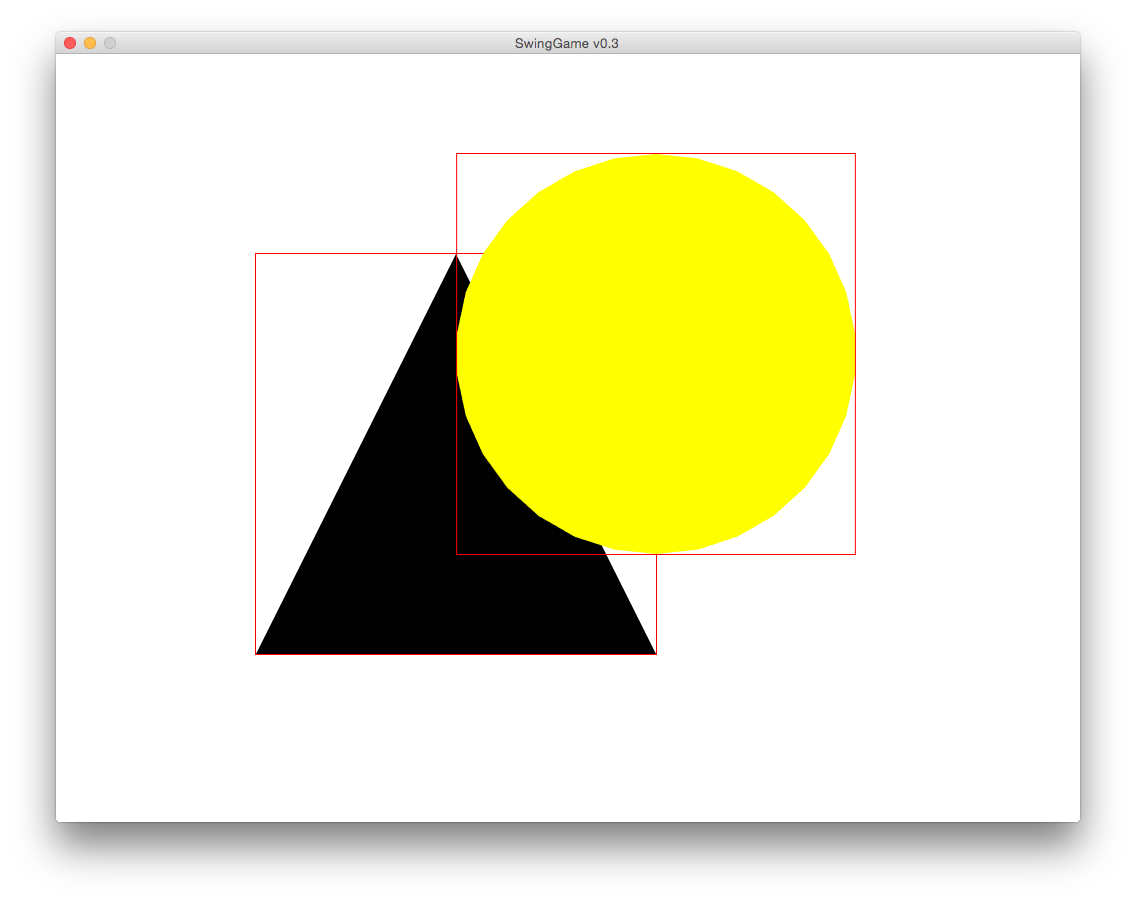
\includegraphics[scale=0.25]{bbcollision}
				\caption{The two bounding boxes intersect and the shapes within are colliding}
				\label{bbcollision}
			\end{figure}
			\begin{figure}[H]
				\centering
				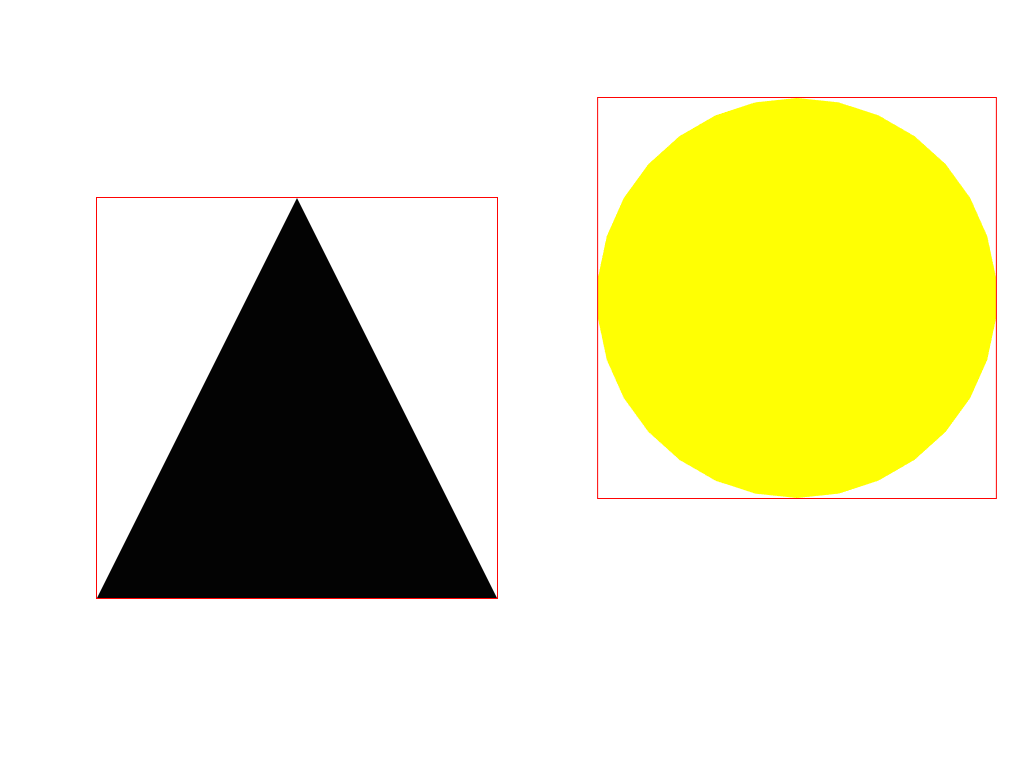
\includegraphics[scale=0.25]{bbnooverlap}
				\caption{The two bounding boxes do not intersect so the shapes within cannot be colliding}
				\label{bbnooverlap}
			\end{figure}
			\begin{figure}[H]
				\centering
				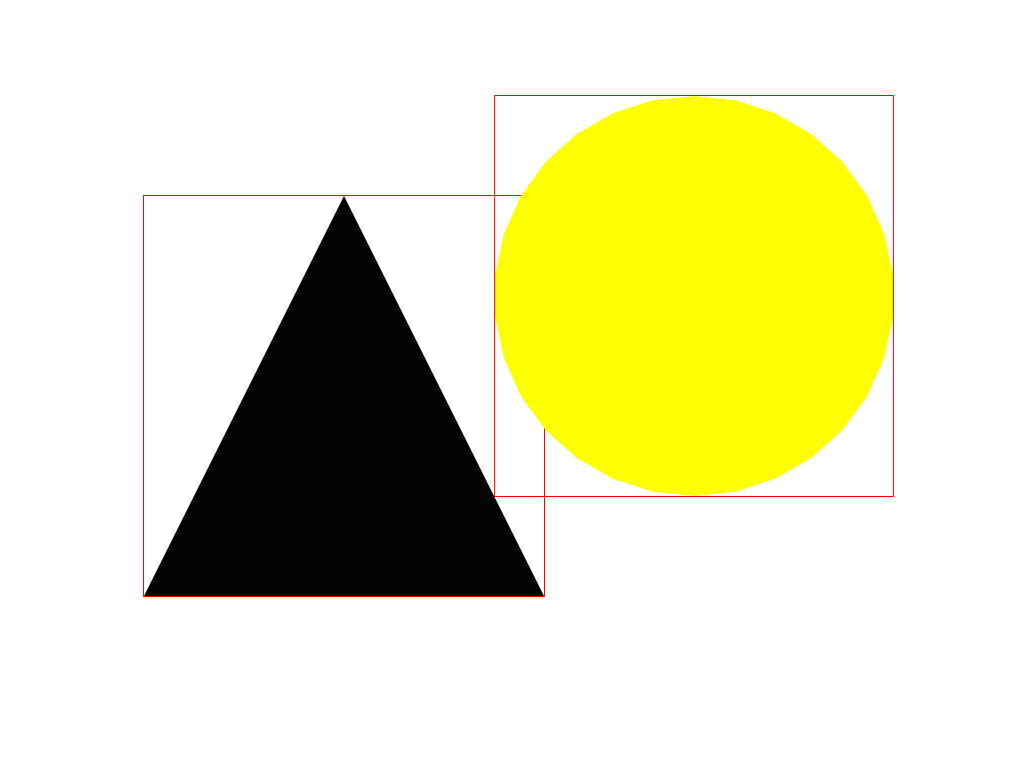
\includegraphics[scale=0.25]{bbnocollision}
				\caption{The two bounding boxes intersect but the shapes within are not colliding}
				\label{bbnocollision}
			\end{figure}
			
			The first iteration of the narrow phase used the very simple concept of line intersections to check for collisions. If any line from shape A is intersecting any line from shape B then A and B are colliding. To check if two lines, A and B are intersecting they are first checked for an intersection assuming the lines are infinitely long. If the two infinite lines intersect then $u_{a}$ is given which is the proportion along line A that the intersection occurred. Similarly $u_{b}$ is the proportion along line B that the intersection occurred. If $u_{a}$ is 0.5 then the intersection occurred halfway along line A. Therefore if both $u_{a}$ and $u_{b}$ are between 0 and 1 then the intersection occurred on lines A and B so the two lines intersect. $u_{a}$ and $u_{b}$ can be found using the equations in Figure \ref{lineintersectionequation}. If the denominator of those equations is 0 then the two lines are parallel so cannot intersect.
			
			\begin{figure}[H]
				\centering
				$x_{A_{1}}$ = The x coordinate of the start of line A
				
				$x_{A_{2}}$ = The x coordinate of the end of line A
				
				$x_{B_{1}}$ = The x coordinate of the start of line B
				
				$x_{B_{2}}$ = The x coordinate of the end of line B
				
				$y_{A_{1}}$ = The y coordinate of the start of line A
				
				$y_{A_{2}}$ = The y coordinate of the end of line A
				
				$y_{B_{1}}$ = The y coordinate of the start of line B
				
				$y_{B_{2}}$ = The y coordinate of the end of line B
				
				$u_{a}$ = The proportion along line A at which lines A and B intersect
				
				$u_{b}$ = The proportion along line B at which lines A and B intersect
				\begin{displaymath}
				u_{a} = \frac
				{(x_{B_{2}}–x_{B_{1}})(y_{A_{1}}–y_{B_{1}})–(y_{B_{2}}–y_{B_{1}})(x_{A_{1}}–x_{B_{1}})}
				{(y_{B_{2}}–y_{B_{1}})(x_{A_{2}}–x_{A_{1}})–(x_{B_{2}}–x_{B_{1}})(y_{A_{2}}–y_{A_{1}})}
				\end{displaymath}
				\begin{displaymath}
				u_{b} = \frac
				{(x_{A_{2}}–x_{A_{1}})(y_{A_{1}}–y_{B_{1}})–(y_{A_{2}}–y_{A_{1}})(x_{A_{1}}–x_{B_{1}})}
				{(y_{B_{2}}–y_{B_{1}})(x_{A_{2}}–x_{A_{1}})–(x_{B_{2}}–x_{B_{1}})(y_{A_{2}}–y_{A_{1}})}
				\end{displaymath}
				\caption{Equations to find the intersection point of lines A and B \cite{linecollisionsite}}
				\label{lineintersectionequation}
			\end{figure}
			
			This worked very well for most cases but caused problems if one shape was completely inside another (Figure \ref{lineintersectionproblem}). In this situation the framework would need to report that a collision was detected to the game as in most cases one object should not be inside another. This situation could arise if in one cycle of the game an object moved from completely outside an obstacle to completely inside an obstacle, and the game would need to know this has happened to react to it.
			
			\begin{figure}[H]
				\centering
				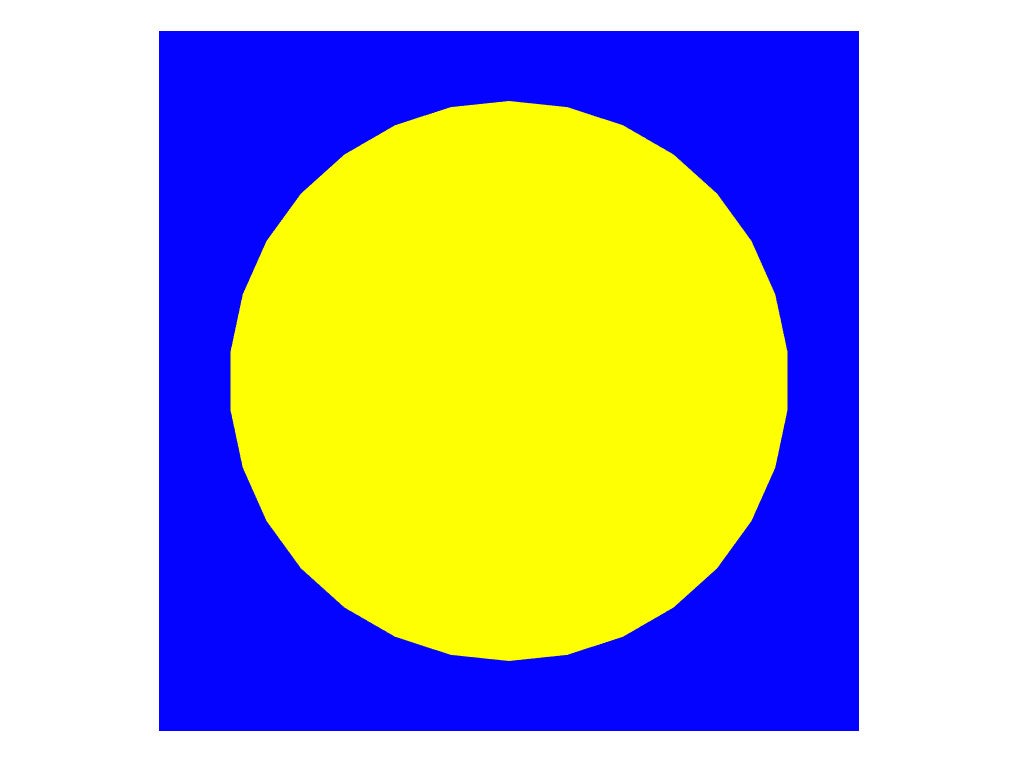
\includegraphics[scale=0.25]{lineintersectionproblem}
				\caption{The circle is completely inside the square meaning no collision is detected}
				\label{lineintersectionproblem}
			\end{figure}
			
			The solution to this problem was to use a different method for the narrow phase collision detection. It was decided to use Separating Axis Theorum (SAT) \cite{sattutorial} because SAT works for all convex shapes which is what the game framework uses and SAT is based on vector maths which is very efficient. 
			
			According to SAT if a line can be drawn between two shapes then they cannot be colliding. This is shown in Figure \ref{satlines}. To check for this algorithmically an axis must be found where if the two shapes are projected onto that axis those projections do not overlap. If that axis can be found then the two shapes are not colliding, if it cannot be found then the shapes are colliding. This is shown in Figure \ref{nsatprojections}. When attempting to find an axis in which the projections of two shapes do not overlap there is only a finite list of axis which need to be checked. These axis correspond to the normals of each line of the two shapes \cite{sattutorial}.
			
			\begin{figure}[H]
				\centering
				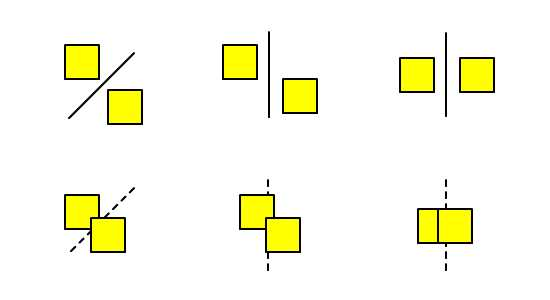
\includegraphics[scale=0.65]{satlines}
				\caption{On the top row the shapes are not colliding so a line can be drawn between them. On the bottom row the shapes are colliding so no lines can be drawn between them. \cite{sattutorial}}
				\label{satlines}
			\end{figure}
			
			\begin{figure}[H]
				\centering
				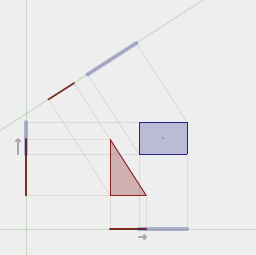
\includegraphics[scale=0.65]{nsatprojnocollide}
				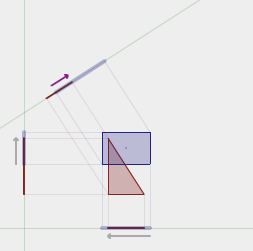
\includegraphics[scale=0.66]{nsatprojcollide}
				\caption{In the left image there is an axis in which the projections do not overlap so the shapes cannot be colliding. In the right image there is no axis in which the projections do not overlap so the shapes must be colliding. \cite{nsattutorial}}
				\label{nsatprojections}
			\end{figure}
			
			To produce the projection of a shape onto the axis each point of the shape is projected onto a point on the axis. If both the point and the axis are represented as vectors then this projection can be calculated using the dot product of the two vectors \cite{sattutorial} which is explained in Figure \ref{dotproduct}. The minimum and maximum of these projected points is kept for each shape. These values are then used to check if the projections overlap with the expression in Figure \ref{projectionoverlapexpression}. This expression is checking if the maximum point of either projection is inside the other projection, if this is the case then the projections overlap.
			
			\begin{figure}[H]
				\centering
				\begin{displaymath}
					A \cdot B = A_x \times B_x + A_y \times B_y
				\end{displaymath}
				\caption{The dot product of two 2D vectors A and B}
				\label{dotproduct}
			\end{figure}
			
			\begin{figure}[H]
				\centering
				\begin{displaymath}
					(A_{max} \geq B_{min} \land A_{max} \leq B_{max}) \lor (B_{max} \geq A_{min} \land B_{max} \leq A_{max})
				\end{displaymath}
				\caption{Boolean expression to check if projections from two shapes, A and B are overlapping}
				\label{projectionoverlapexpression}
			\end{figure}
			
			To summarise, SAT checks for collisions by checking for overlaps in a list of axis which corresponds to the normals present on each shape. Overlaps are checked for by projecting each shape onto the current axis and checking if the projections overlap. If any axis has projections that do not overlap then the shapes are not colliding.
			
		\subsection{SwingGame}
		Modules made for SwingGame were bespoke tasks relevant only to that particular game.
			\subsubsection{Levels}
			The levels for SwingGame were made to be completely data driven. The files that define the levels were written in XML and are read using the pugixml library. It was decided to have SwingGame load all valid level files which are present at runtime to not only facilitate the easy addition of new levels but to also allow users to create their own levels which can be loaded in.
			
			Levels were implemented by simply having one player per level and a list of obstacles which the player can collide with and swing on. Every update cycle the level is checked for completion by checking if the player is completely inside the goal and it is checked for failure by checking if the player is completely outside the window boundaries. A list of keys was added to levels which blocks the player from the goal while the list is not empty. When the player collides with a key it is removed from the list so a player must collect all keys to unlock the goal of the level. One level from SwingGame is shown in Figure \ref{levelexample}. Images of each level can be found in Appendix A.
			
			\begin{figure}[H]
				\centering
				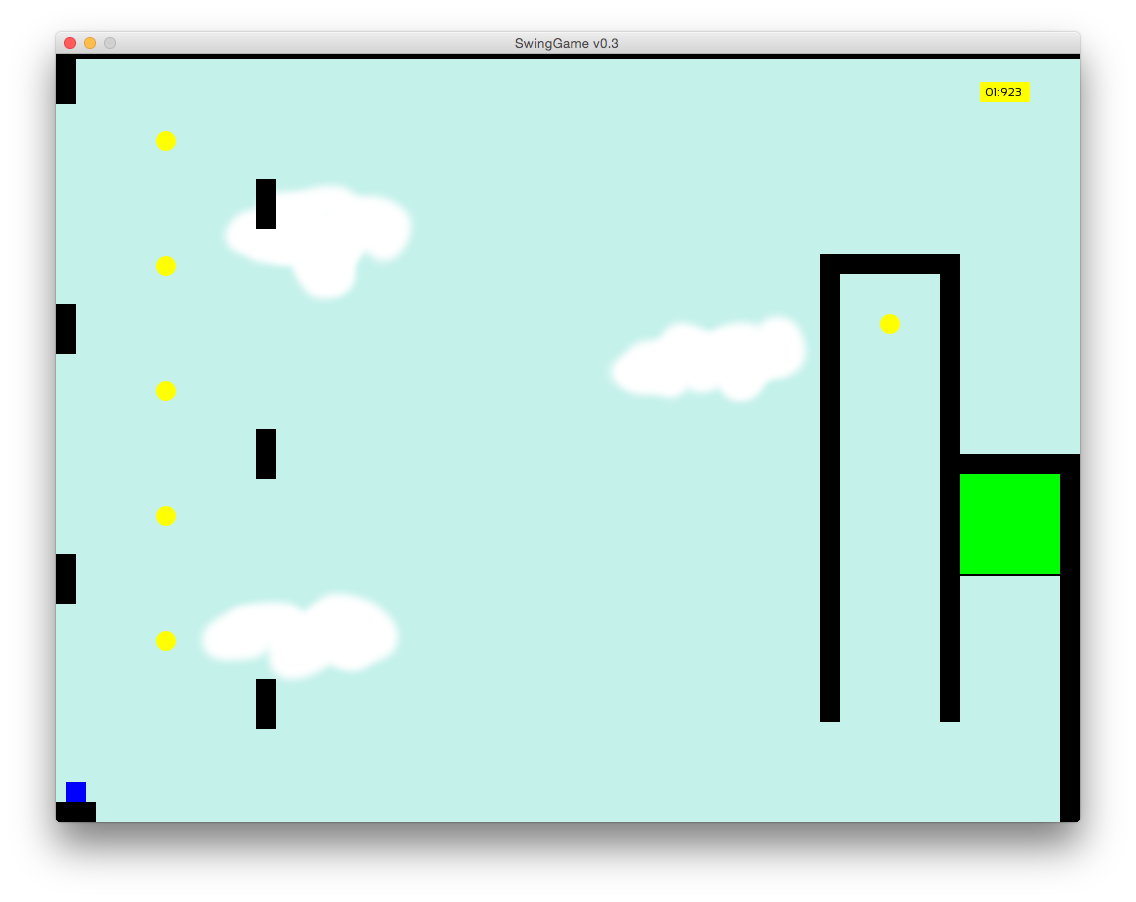
\includegraphics[scale=0.25]{level8}
				\caption{Level 8 of SwingGame. The blue square is the player, black shapes are obstacles, the green square is the goal and the yellow circles are keys.}
				\label{levelexample}
			\end{figure}
			\subsubsection{Gameplay Mechanics}
			The gameplay mechanics of SwingGame are the set of actions that a player can do. Most of these had fairly simple implementations, for example when the jump button is pressed while the player is on a swing that can be jumped from then detach them from the swing and give them an upwards velocity. The only mechanic with an interesting implementation is firing a swing.
			
			When a swing is fired the current position of the mouse is used as the aim point for that swing. SwingGame looks for the first obstacle on the line from the players current position to the aim point to anchor the swing to. When anchoring a swing a small gap is left between the end of the swing and the obstacle to ensure collisions are not constantly detected between the end of the swing and the obstacle. This is shown in Figure \ref{anchorGap}.
			
			\begin{figure}[H]
				\centering
				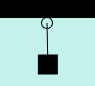
\includegraphics{anchorGap}
				\caption{A swing anchored to an obstacle, the circle shows the anchor gap between the swing and the obstacle.}
				\label{anchorGap}
			\end{figure}
			
			The way this gap was initially implemented was by creating a line from the players position to the aim point and finding the first intersection along that line with any obstacles in the level. When the first intersection is found the anchor point is set to the position on that line a fixed distance before the intersection point, this distance is known as the anchor gap. This implementation had the problem that if a swing was close to parallel to an obstacle the anchor point would still be too close to the obstacle even after moving back along the line by the anchor gap. This is shown in Figure \ref{anchorProblem}.
			
			\begin{figure}[H]
				\centering
				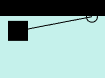
\includegraphics{anchorProblem}
				\caption{A swing anchored to an obstacle where the swing is closer than the anchor gap to the obstacle.}
				\label{anchorProblem}
			\end{figure}
			
			The solution implemented for this problem was to check each point along the line from the players position to the aim point until a valid anchor point is found. Starting at the players position at each pixel along this line a circle is created with a radius of the anchor gap. If this circle does not collide with any obstacle the next pixel along the line is checked. If the circle does collide with an obstacle then that pixel is set as the anchor point for the swing.
			
			\subsubsection{Physics}
			Initially the physics module for this project was intended to be part of the game framework as a very generic simulation of real world physics. This implementation was going to be based on applying forces to the physical bodies such as the normal force from obstacles the body collides with and the tension force from the swing. Eventually it was decided that the complexity of this implementation was not worth the benefit it would bring since there are very little games that require physics accurate to the real world. Instead the physics module was made within SwingGame and is very specific to the physics of that game.
			
			The physics of SwingGame is based on a small set of rules. One of these is that when the player is not attached to a swing they accelerate downwards due to gravity. Another is that when the player collides with an obstacle the velocity of the player should be reflected based on the orientation of the collision surface. For example a player colliding with a horizontal surface should have the y component of their velocity reflected. To calculate the reflection of velocity for an arbitrary oriented surface first calculate the components of velocity perpendicular and parallel to that surface ($v_{perp}$ and $v_{par}$ respectively ). This is done by projecting the velocity vector onto those direction vectors using the dot product. Scale these components by values for friction ($f$) and elasticity ($e$) and combine them into the response vector. Calculate the new velocity by subtracting this response from the old velocity. This is shown by the equation in Figure \ref{collisionResponse}.
			
			\begin{figure}[H]
				\centering
				\begin{displaymath}
					0 \leq e \leq 1
				\end{displaymath}
				\begin{displaymath}
					0 \leq f \leq 1
				\end{displaymath}
				\begin{displaymath}
					vel_{new} = vel_{old} - ((v_{perp} \times (1+e)) + (v_{par} \times f))
				\end{displaymath}
				\caption{Equation to calculate the reflected velocity after colliding with a surface of arbitrary orientation.}
				\label{collisionResponse}
			\end{figure}
			
			The last rule for physics is that when the player is on a swing apply the component of gravity which is perpendicular to the direction of the swing. This is what provides the arc of the swing. It means that when the swing is completely horizontal the full acceleration of gravity is applied downwards. As the player swings towards their lowest point on the swing (equilibrium position \cite{pendulumWiki}) the magnitude of the acceleration decreases to zero while its direction remains perpendicular to the swing. This model produces a swing motion with all the important properties of a true pendulum. 
			\begin{itemize}
				\item{Acceleration is at a minimum and velocity is at a maximum at the equilibrium position}
				\item{Velocity is at a minimum at the top of the swing}
				\item{Acceleration is at a maximum when the swing is horizontal}
			\end{itemize}
			Figure \ref{swingingMotion} shows these values at various points during swinging.
			
			\begin{figure}[H]
				\centering
				\begin{subfigure}[b]{1\textwidth}
				\centering
		        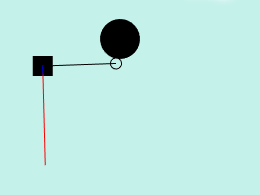
\includegraphics[scale=0.4]{swingingMotionLeftTop}
		        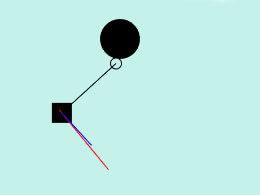
\includegraphics[scale=0.4]{swingingMotionLeftLower}
		        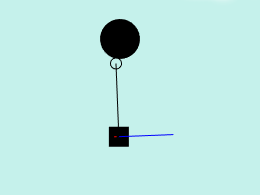
\includegraphics[scale=0.4]{swingingMotionBottom}
		        \end{subfigure}
		        
		        \vspace{3 pt}
		        
				\begin{subfigure}[b]{1\textwidth}
				\centering
		        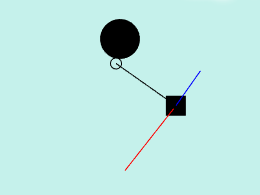
\includegraphics[scale=0.4]{swingingMotionRightLowerUp}
		        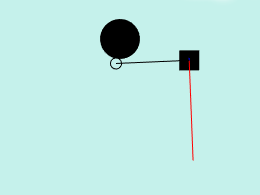
\includegraphics[scale=0.4]{swingingMotionRightTop}
		        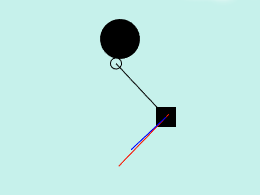
\includegraphics[scale=0.4]{swingingMotionRightLowerDown}
  		        \end{subfigure}
				\caption{Acceleration (red) and velocity (blue) at various stages of a swing.}
				\label{swingingMotion}
			\end{figure}
			
			\subsubsection{Swing Types}
			Three different types of swing were added to SwingGame. One is a rigid swing which bounces off obstacles if it collides with them. This was done by simply flipping the players velocity to point in the opposite direction.
			
			A flexible swing was added which wraps around the obstacles in the level (Figure \ref{swingWrap}). This was achieved by having the flexible swing as a subclass of the rigid swing which behaves differently when it collides with an obstacle. The flexible swing keeps a list of previous anchor points and when it collides with an obstacle it adds the current anchor point to the previous list and sets the point at which the collision occurred as the current anchor point. This swing also needed to know when to unwrap itself, this was achieved by creating a triangle from the players current position, the current anchor point and the previous anchor point. If this triangle is colliding with any obstacles then the swing does not need to unwrap, if it is not colliding then it does need to unwrap. This is shown in Figure \ref{swingUnwrap}.
			
			\begin{figure}[H]
				\centering
				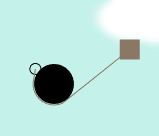
\includegraphics{swingWrap}
				\caption{The flexible swing wrapping around a circle obstacle}
				\label{swingWrap}
			\end{figure}
			
			\begin{figure}[H]
				\centering
				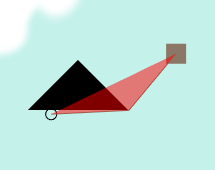
\includegraphics[scale=0.6]{swingUnwrapNo}
				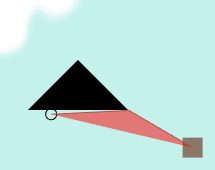
\includegraphics[scale=0.6]{swingUnwrapYes}
				\caption{The flexible swing unwrapping. In the left image the red triangle is colliding with an obstacle so the swing should not unwrap. In the right image the red triangle is not colliding with anything so the swing should unwrap.}
				\label{swingUnwrap}
			\end{figure}
			
			The final swing type added was a pulling swing which reels the player in towards the swings anchor point. This was done by simply removing the players current velocity when they attach and then altering gravity to be an acceleration towards the anchor point.
		

\chapter{Evaluation}
This chapter discusses how the project was evaluated, including both SwingGame and the game framework.
	\section{External Testing}
	SwingGame was evaluated by having colleagues play different builds of the game. This was initially a testing process where bugs found in one build would be fixed for the next. Three of these builds were released though only the first and third received much attention. After the third build was released a survey was advertised to attempt to gain information about what the players liked and disliked about SwingGame.
		\subsection{Feedback}
		This Section details the feedback received from the player survey.
			\subsubsection{Clarity of the Game}
			It was important that players understood what they were supposed to achieve and how to do achieve it. When asked how clear it was to play the game 71.43\% responses claimed it was clear while the rest answered with very clear.
			\subsubsection{Level Completion}
			Knowing how many players attempted and completed each level was useful to gauge how the game retained interest and how difficult each level was. The following table shows the percentage of respondents which attempted each level, and how many completed each level.
			
			\begin{figure}[H]
			\begin{tabular}[H]{ l || c | c | c}
				Level & \specialcell{Percentage\\of attempts} & \specialcell{Percentage\\of completions} & \specialcell{Percentage\\of failed attempts} \\
				\hline
				1 & 85.71 & 85.71 & 0.00 \\
				2 & 85.71 & 85.71 & 0.00 \\
				3 & 71.43 & 71.43 & 0.00 \\
				4 & 71.43 & 71.43 & 0.00 \\
				5 & 57.14 & 57.14 & 0.00 \\
				6 & 71.43 & 14.29 & 57.14 \\
				7 & 57.14 & 42.86 & 14.28 \\
				8 & 42.86 & 28.57 & 14.29 \\
				9 & 42.86 & 14.29 & 28.57 \\
			\end{tabular}
			\end{figure}
			
			These results show that interest starts to drop as soon as level three and less than half of the respondents attempted all nine levels. The first five levels proved to be straightforward since all respondents who attempted them were able to complete them but the remaining levels forced some respondents to give up. Judging from the percentage of failed attempts level six (Figure \ref{level6}) was the most difficult.
				
			\subsubsection{Level Enjoyment}
			In order to know which types of levels players enjoyed the most they were asked to state their most and least favourite levels. The following table shows for each level the percentage of respondents which claimed that level was their most or least favourite.
			
			\begin{figure}[H]
			\begin{tabular}[H]{ l || c | c }
				Level & \specialcell{Percentage of\\favourites} & \specialcell{Percentage of\\least favourites} \\
				\hline
		        1 & 0.00 & 0.00 \\
		        2 & 0.00 & 14.29 \\
		        3 & 14.29 & 0.00 \\
		        4 & 28.57 & 14.29 \\
		        5 & 28.57 & 14.29 \\
		        6 & 0.00 & 14.29 \\
		        7 & 14.29 & 14.29 \\
		        8 & 0.00 & 14.29 \\
		        9 & 14.29 & 14.29 \\
			\end{tabular}
			\end{figure}
			
			The only information which was gained from these results was that no level was universally loved nor hated, but levels four and five (Figures \ref{level4} and \ref{level5}) were liked slightly more than the rest.
			
			\subsubsection{Swing Type Preference}
			The respondents were asked to rank each swing in order of enjoyment in an attempt to find out which was the most fun to use. The following table shows the rankings for each swing with one being the most enjoyable.
			
			\begin{figure}[H]
			\begin{tabular}[H]{ l || c | c | c }
				Swing Type & \specialcell{Percentage of\\rank 1s} & \specialcell{Percentage of\\rank 2s} & \specialcell{Percentage of\\rank 3s} \\
				\hline
		        Rigid & 14.29 & 14.29 & 71.43 \\
		        Flexible & 42.86 & 42.86 & 14.29 \\
		        Pulling & 42.86 & 42.86 & 14.29 \\
			\end{tabular}
			\end{figure}
			
			Using these rankings each swing type was given the following overall score.
			
			\begin{figure}[H]
			\begin{tabular}[H]{ l || c }
				Swing Type & Score \\
				\hline
				Rigid & 1.43 \\
				Flexible & 2.29 \\
				Pulling & 2.29 \\
			\end{tabular}
			\end{figure}
			
			These results simply show that the rigid swing is the least fun of all three swing types.
			
			\subsubsection{Overall Game Enjoyment}
			Players were asked how enjoyable they found the game using a five point scale from very boring to very enjoyable. 85.71\% of respondents stated they found the game enjoyable with the rest claiming they found it neither enjoyable nor boring.
			
	\section{Use In Other Projects}
	Since the game framework was intended to be used for multiple projects it should be evaluated based on how effective it has been to use in projects it was not tailor made for. The framework has been used in two other projects so far, each one is detailed in this Section.
		\subsection{Particle System}
		An assignment for the Advanced Computer Graphics course for third years at the University of Manchester was to produce a particle system. The game framework from this project was successfully used to create a particle system for this assignment, using all modules from the framework apart from the graphics and collision modules. These modules were not used as they work only in 2D but the particle system was in 3D. Rendering in this project was done using OpenGL instead which the framework was able to handle. During this project functionality for a 3D camera which can be controlled to move around the scene and look in different directions was added to the game framework.
		
		\begin{figure}[H]
			\centerline{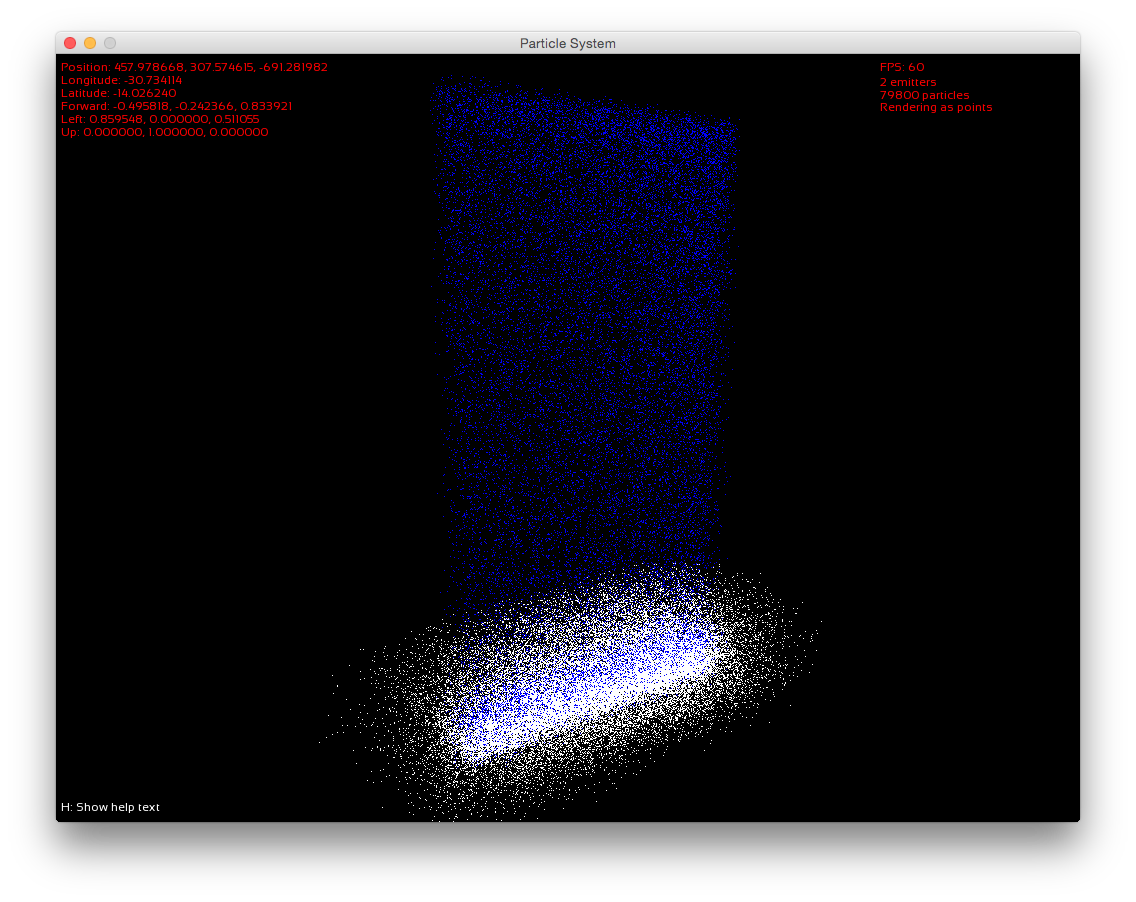
\includegraphics[width=1.5\textwidth]{particlesystem}}
			\caption{Particle system rendering a waterfall}
			\label{particlesystem}
		\end{figure}
		
		\subsection{Tick Tack Toe}
		Tick Tack Toe is another game currently being developed on top of the game framework. It features a tick (the arachnid) which is being attacked by a hoard of toes trying to squash it. The tick can fight back against the toes by throwing thumb tacks at them. This game uses all modules of the game framework and the basic gameplay for it was completed in one day thanks to the functionality provided by the framework. So far in this project the event system of the game framework has been changed to use the Observer design pattern and functionality has been added to the graphics module to allow animated game objects.
		
		\begin{figure}[H]
			\centering
			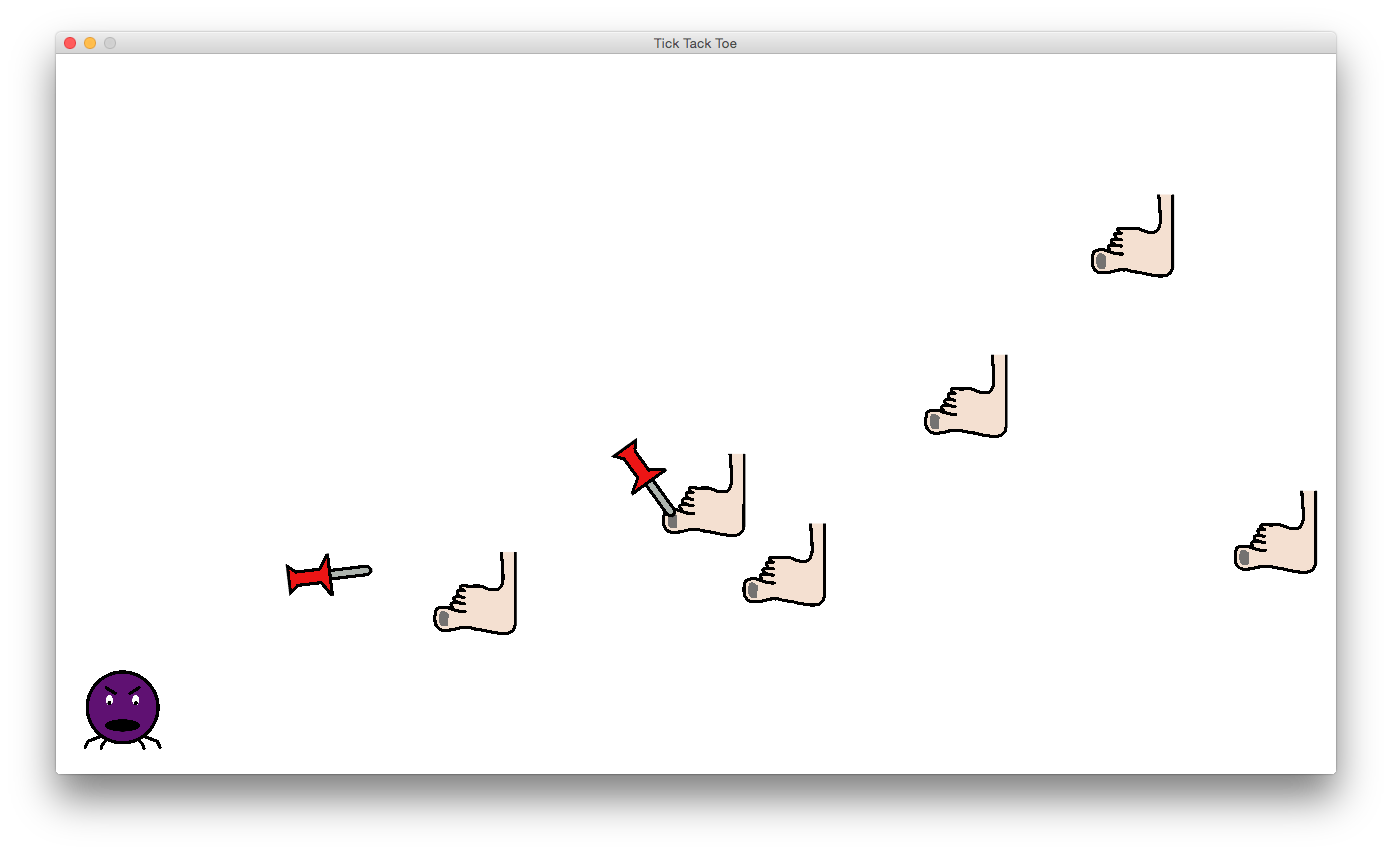
\includegraphics[scale=0.25]{ticktacktoe}
			\caption{Tick Tack Toe in its current state}
			\label{ticktacktoe}
		\end{figure}
	

\chapter{Reflection and Conclusion}
This chapter discusses what went right and what went wrong in this project. It explains whether the objectives were fulfilled and what would be done differently if the project were to be undertaken again.
	\section{Objectives}
	The objectives of the framework produced were to be reusable, extensible and easy to use. I think the framework succeeds in all these regards given its use in other projects. Each project was implemented without having to fight with the framework to get it to work, and each managed to add extra features which were not insubstantial. It could be said that this is the case because the person working on the project is the person who built the framework but it was only ever intended to be used on personal projects so I do not believe this is relevant.
	
	SwingGame was intended to show that the framework can produce a working and finished game and had the side objective of being fun and engaging. It definitely succeeded in showing the worth of the game framework and was somewhat successful at being a fun game. From the player feedback survey it is apparent that players find the game enjoyable but judging from the percentage of people who attempted all levels the game did not retain most players attention for all nine short levels. I feel that this can partly be explained by the look of the game, the focus of the project was never on looking good. This resulted in text only menus and graphics which consisted of simple one colour shapes. This made the game look quite amateur even if the the motion and mechanics had the right feel I was going for.
	
	\section{Lessons Learned}
	If I were to do this project again there are some things I would do differently, the main being not over engineering things. When creating the SFML abstraction layer I spent a lot of time creating a subclass for each SFML class used when a simple typedef would have achieved the same results. I could then have just changed the typedef into a true class when additional functionality was required.
	
	Another example of this is the time wasted when researching how to implement a physics model accurate to the real world. While I did eventually decide to use a much simpler model I should have known from the start that my original idea was way out of scope and looking into it was ultimately pointless.
	
	While creating SwingGame I made no effort to keep the source of the game separate from the framework itself. This lead to a messy situation when I began other projects as I had to isolate what was part of the framework and what was not. From this I learned that when making a generic library it should be kept as a separate project from anything being made alongside that library.
	
	Another lesson learned during this project is that of self motivation. There were large periods of time where I did no work on the project because I felt like the next thing planned would be boring and there were no looming deadlines to force me to work. Eventually I made myself get on with it so I could not only play the finished project but be able to show it off in its best possible state. If I had not done this I believe the game would have been a very rushed at the last minute and a much worse game because of that.
	
	\section{Future Improvements}
	There are many improvements I could make to SwingGame in the future. The most obvious being adding in better art and even animations to make the game look a lot more professional. Another obvious addition would be audio, both ambient background music and sound effects for events that happen in the game. Beyond that extra functionality could also be added to SwingGame, more advanced level features like moving obstacles or teleporters which transport the player to another location could allow for much more diverse levels and puzzles. The game can also always be extended by adding more levels, though I feel my abilities as a level designer would not lead to much better levels than the current set.
	
	I have many more ideas for games I could make with the framework I produced. I imagine each of these will have the opportunity to discover extra features which could be added to the framework. I already have some in mind such as a system for mouse driven user interfaces which have a much more professional feel than the current text driven ones. Some more useful features would be an audio module and a system to rebind inputs to different buttons and keys.
	
	\section{Source Code}
	The source code for both SwingGame and the game framework built in this project has been released under the MIT license. SwingGame and the framework as it was built for SwingGame can be found at \url{https://www.github.com/sizlo/SwingGame}. Ongoing development to the game framework can be found at \url{https://www.github.com/sizlo/TimGameLib}.
	
	\begin{appendices}
		\chapter{Appendix A: The Levels of SwingGame}
		\begin{figure}[H]
			\centering
			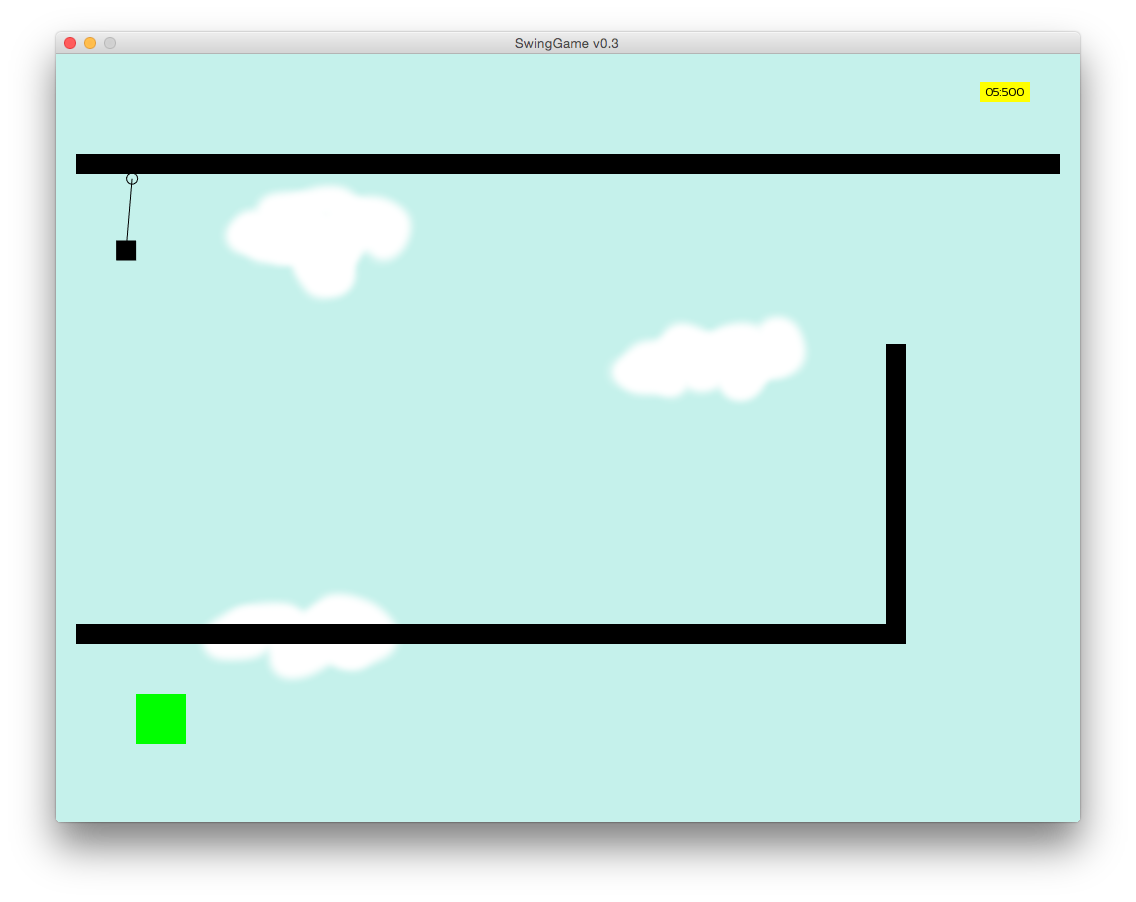
\includegraphics[scale=0.25]{level1}
			\caption{Level 1 of SwingGame}
			\label{level1}
		\end{figure}
		\begin{figure}[H]
			\centering
			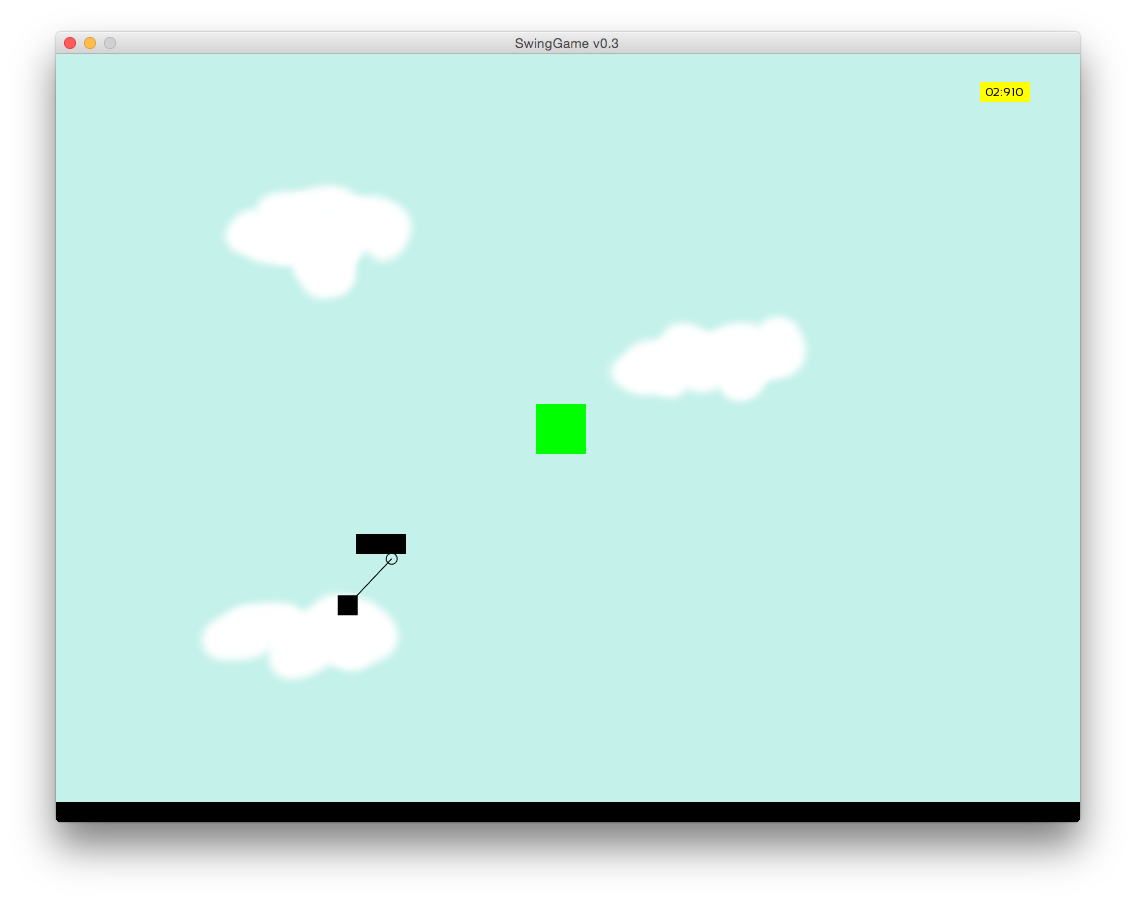
\includegraphics[scale=0.25]{level2}
			\caption{Level 2 of SwingGame}
			\label{level2}
		\end{figure}
		\begin{figure}[H]
			\centering
			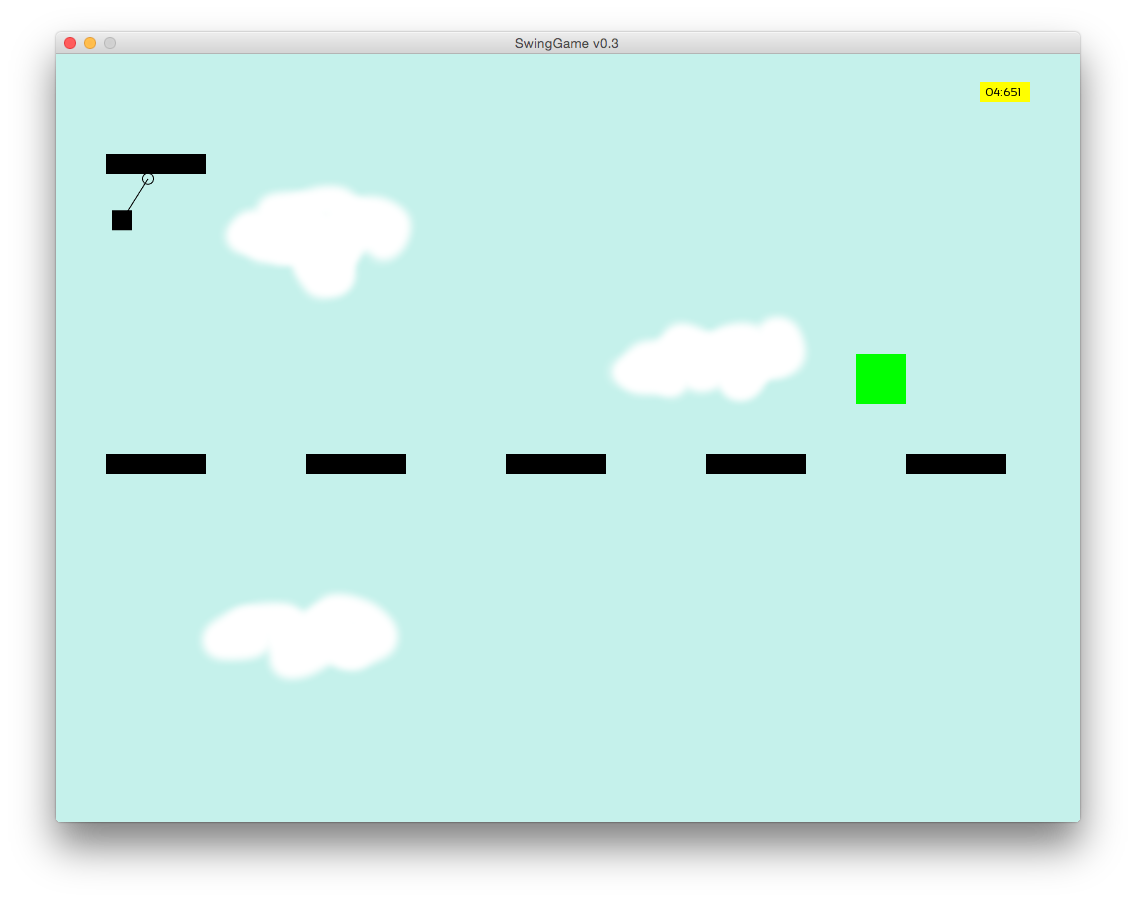
\includegraphics[scale=0.25]{level3}
			\caption{Level 3 of SwingGame}
			\label{level3}
		\end{figure}
		\begin{figure}[H]
			\centering
			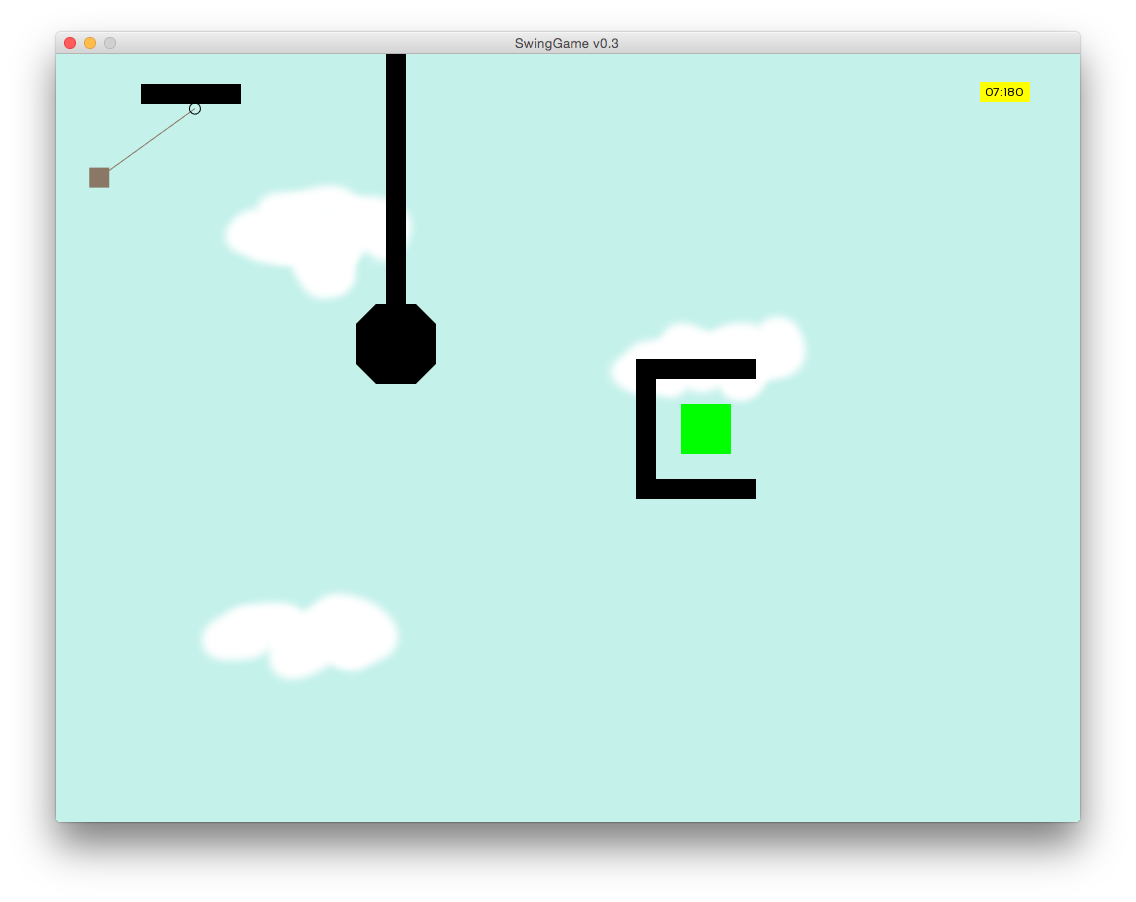
\includegraphics[scale=0.25]{level4}
			\caption{Level 4 of SwingGame}
			\label{level4}
		\end{figure}
		\begin{figure}[H]
			\centering
			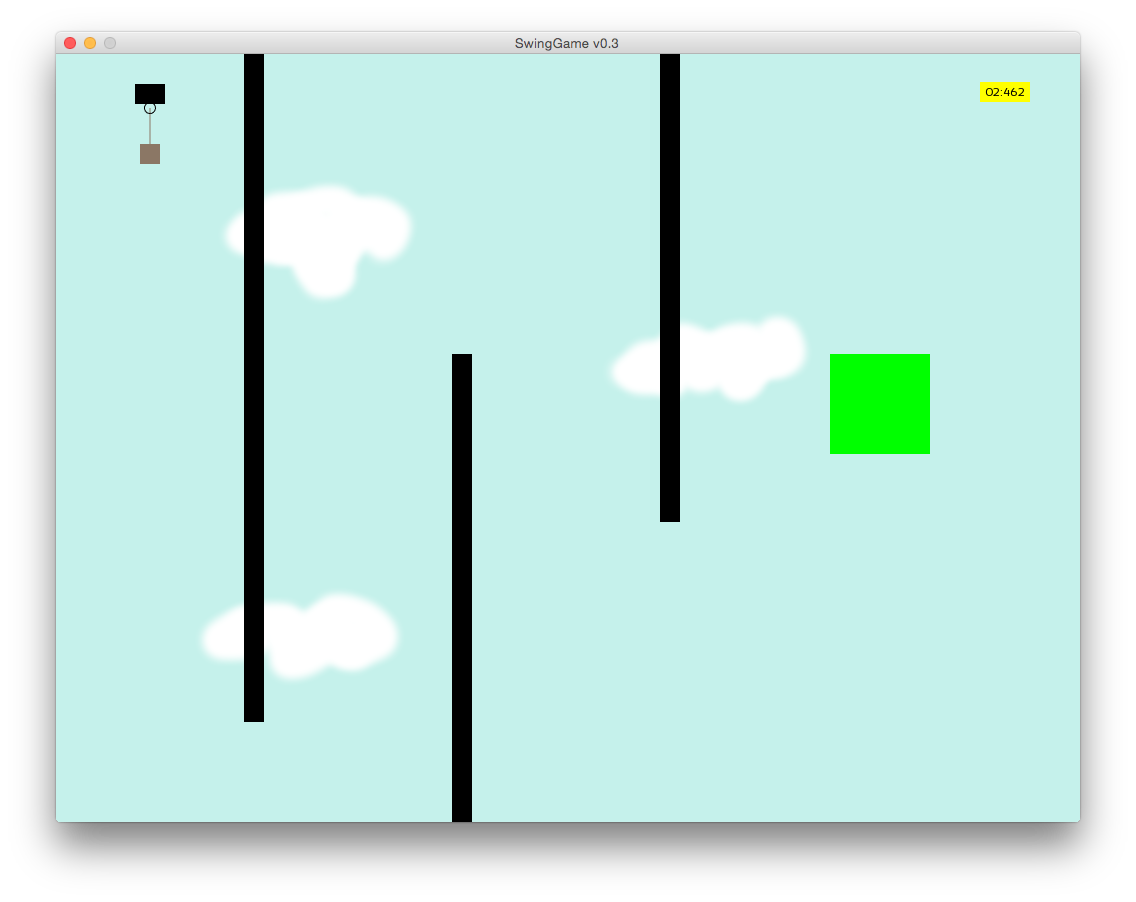
\includegraphics[scale=0.25]{level5}
			\caption{Level 5 of SwingGame}
			\label{level5}
		\end{figure}
		\begin{figure}[H]
			\centering
			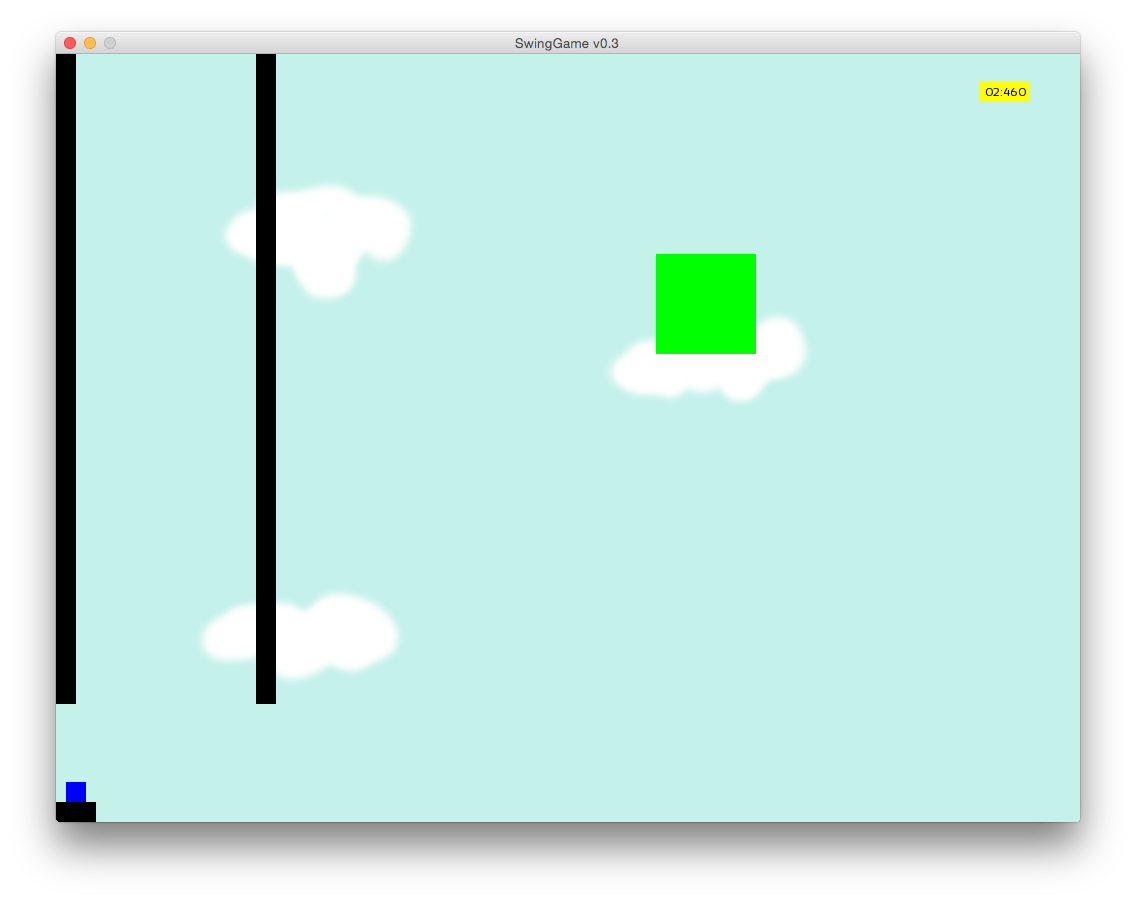
\includegraphics[scale=0.25]{level6}
			\caption{Level 6 of SwingGame}
			\label{level6}
		\end{figure}
		\begin{figure}[H]
			\centering
			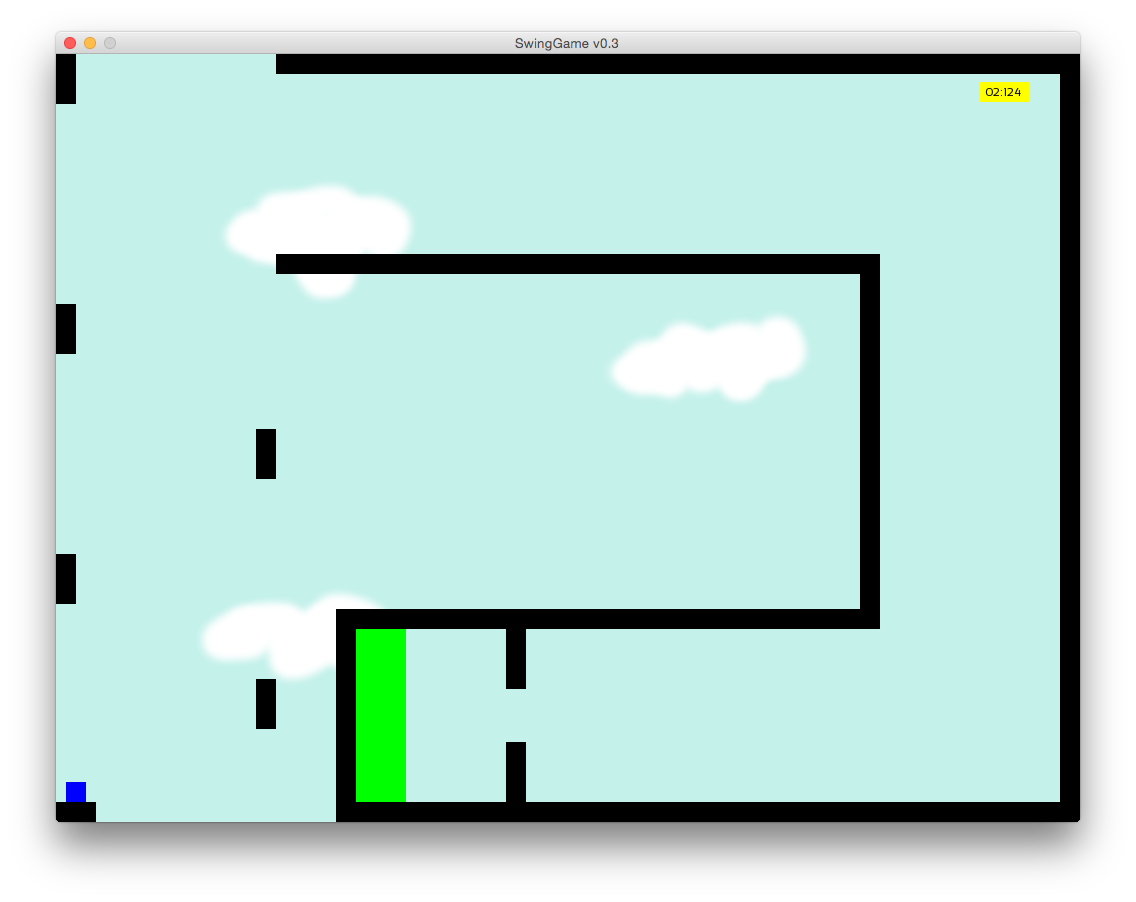
\includegraphics[scale=0.25]{level7}
			\caption{Level 7 of SwingGame}
			\label{level7}
		\end{figure}
		\begin{figure}[H]
			\centering
			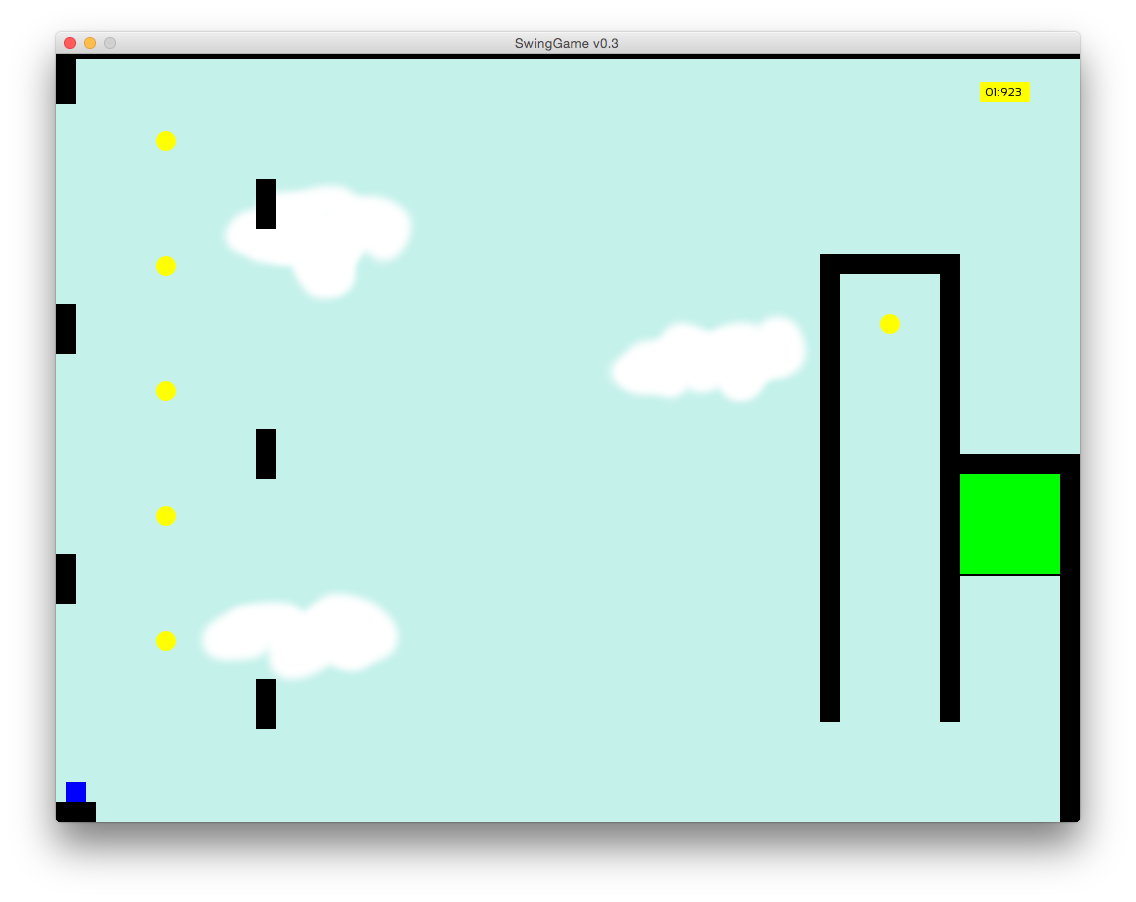
\includegraphics[scale=0.25]{level8}
			\caption{Level 8 of SwingGame}
			\label{level8}
		\end{figure}
		\begin{figure}[H]
			\centering
			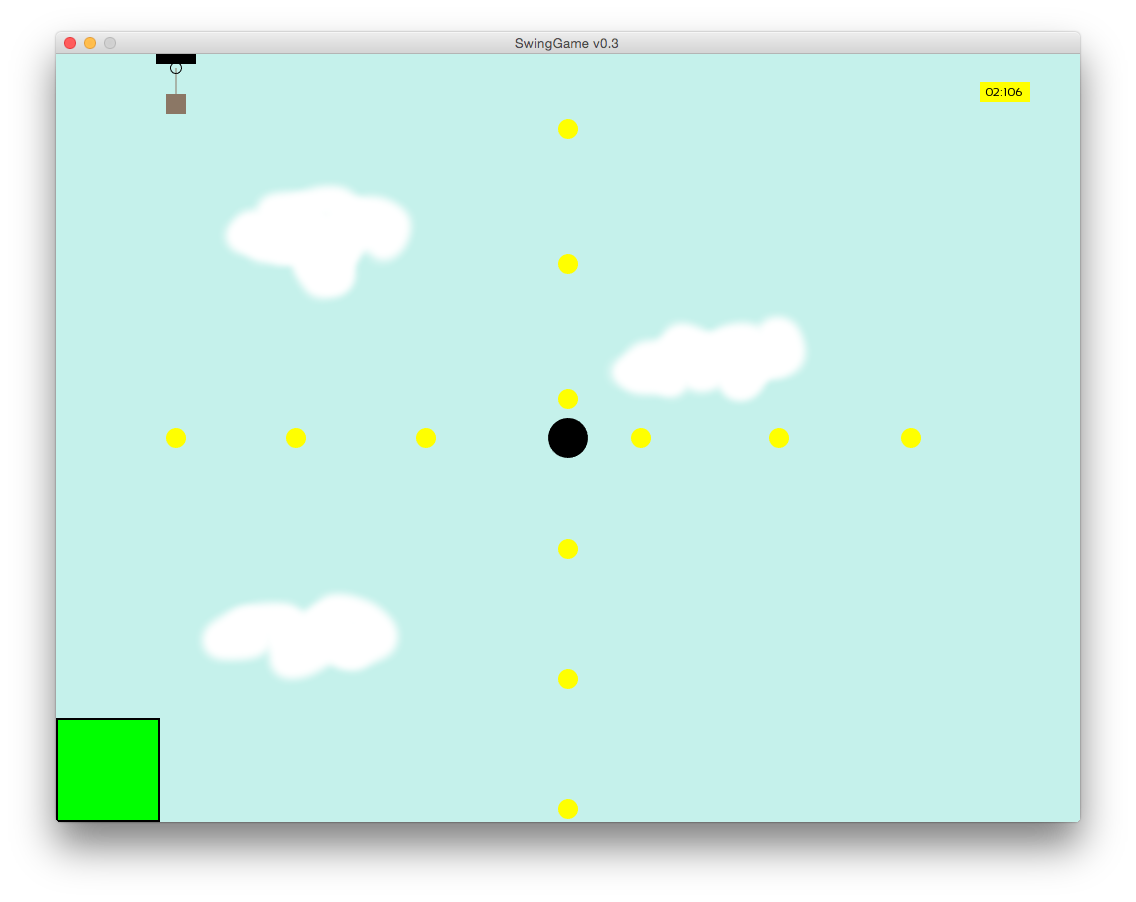
\includegraphics[scale=0.25]{level9}
			\caption{Level 9 of SwingGame}
			\label{level9}
		\end{figure}
		
	\end{appendices}
	
\bibliographystyle{plain}

\bibliography{sources}

\end{document}          






